\documentclass[bachelor, fontsize=14]{diploma}
\usepackage{xcolor}

\student{Батоян Роберт Левонович}
\group{М8О-407Б-22}
\theme{Отказоустойчивая распределённая платформа мультиканальной гарантированной доставки уведомлений в микросервисной архитектуре}

\supervisor{Булакина Мария Борисовна}
\firstConsultant{Филимонов Николай Сергеевич}
\reviewer{}

\faculty{<<Компьютерные науки и прикладная математика>>}
\department{406}
\speciality{01.03.02 <<Прикладная математика и информатика>>}
\profile{Информатика}

\departmentFullName{Кафедра 406 <<Вычислительная математика и программирование>>}
\headOfDepartment{}

\date{\uline{\hspace{24pt}} июня 2026 года}

\newacronym{grpc}{gRPC}{удалённый вызов процедур по протоколу HTTP/2}
\newacronym{kafka}{Kafka}{распределённая платформа потоковой передачи событий}
\newacronym{api}{API}{программный интерфейс приложения}
\newacronym{dbms}{СУБД}{система управления базами данных}
\newacronym{nosql}{NoSQL}{класс нереляционных систем управления данными}
\newacronym{sql}{SQL}{язык структурированных запросов}
\newacronym{jdbc}{JDBC}{интерфейс доступа Java-приложений к реляционным базам данных}
\newacronym{mongodb}{MongoDB}{документоориентированная NoSQL СУБД}
\newacronym{redis}{Redis}{in-memory хранилище данных типа key-value}
\newacronym{json}{JSON}{текстовый формат обмена структурированными данными}
\newacronym{protobuf}{protobuf}{язык описания контрактов и формат сериализации сообщений}
\newacronym{smtp}{SMTP}{протокол передачи электронной почты}
\newacronym{sms}{SMS}{служба коротких текстовых сообщений}
\newacronym{jvm}{JVM}{виртуальная машина Java}
\newacronym{rps}{RPS}{число запросов или сообщений в секунду}
\newacronym{p95}{p95}{95-й процентиль наблюдаемой величины}
\newacronym{saas}{SaaS}{программное обеспечение, предоставляемое как сервис}
\newacronym{jwt}{JWT}{маркер веб-токена}
\newacronym{tls}{TLS}{протокол криптографической защиты транспортного соединения}
\newacronym{rest}{REST}{архитектурный стиль представления состояния ресурса}
\newacronym{dsl}{DSL}{предметно-ориентированный язык описания}

\newglossaryentry{event}{
    name={Уведомительное событие},
    description={зарегистрированное намерение выполнить доставку сообщения заданной аудитории с определённым шаблоном и полезной нагрузкой}
}

\newglossaryentry{dispatch}{
    name={Запуск доставки},
    description={экземпляр исполнения уведомительного события с фиксированной аудиторией и параметрами отправки}
}

\newglossaryentry{delivery}{
    name={Канальная доставка},
    description={обработка уведомления для конкретного получателя и конкретного канала связи в рамках одного запуска доставки}
}

\newglossaryentry{delivery_history}{
    name={История доставки},
    description={агрегированное представление статусов, позволяющее восстановить путь обработки от входной команды до итогового результата}
}

\newglossaryentry{template_term}{
    name={Шаблон},
    description={версионируемое описание содержимого уведомления для конкретного канала связи}
}

\newglossaryentry{provider}{
    name={Канальный шлюз},
    description={внешний или внутренний компонент, выполняющий фактическую передачу уведомления по выбранному каналу}
}

\newglossaryentry{outbox_pattern}{
    name={transactional outbox},
    description={паттерн надёжной публикации интеграционных сообщений, при котором бизнес-изменение и запись сообщения фиксируются в одной транзакции базы данных}
}

\newglossaryentry{idempotency}{
    name={идемпотентность},
    description={свойство операции, при котором повторный запуск с теми же входными параметрами не приводит к дополнительным побочным эффектам}
}

\newglossaryentry{deduplication}{
    name={дедупликация},
    description={обнаружение и подавление дублирующихся сообщений или операций по устойчивому ключу}
}

\newglossaryentry{redis_deduplication}{
    name={дедупликация через Redis},
    description={техническое подавление повторной обработки sender-команд через атомарную запись TTL-ключа в Redis}
}

\newglossaryentry{retry_term}{
    name={повторная попытка},
    description={контролируемое повторное выполнение операции после временной ошибки}
}

\newglossaryentry{fallback_routing}{
    name={fallback-маршрутизация},
    description={переназначение доставки в альтернативный канал связи после окончательной ошибки или исчерпания повторов в исходном канале}
}

\newglossaryentry{cancellation_mark}{
    name={отметка отмены},
    description={TTL-ключ в Redis, фиксирующий отмену dispatch или delivery и используемый sender-сервисами перед фактической отправкой}
}

\newglossaryentry{history_writer}{
    name={history-writer},
    description={сервис, который потребляет статусные события доставки и записывает append-only историю в ClickHouse}
}

\newglossaryentry{eventual_consistency}{
    name={eventual consistency},
    description={модель согласованности распределённой системы, в которой синхронизация состояний между сервисами происходит за конечное, но не мгновенное время}
}

\newglossaryentry{at_least_once}{
    name={at-least-once delivery},
    description={модель доставки сообщений, при которой каждое сообщение доставляется получателю не менее одного раза; возможны дубликаты, которые должны обрабатываться на уровне приложения}
}

\newglossaryentry{fault_tolerance}{
    name={fault tolerance},
    description={свойство системы сохранять работоспособность при частичных отказах компонентов}
}

\newglossaryentry{document_model}{
    name={документоориентированная модель данных},
    description={модель хранения, в которой связанные атрибуты предметной сущности размещаются в одном документе и обрабатываются как единое целое}
}


\addbibresource{main.bib}
\newcommand{\assumption}[1]{\textcolor{red}{\textbf{Допущение:} #1}}

\begin{document}
    \maketitle
    \setcounter{page}{2}

    \abstract

\keywords{РАСПРЕДЕЛЁННЫЕ СИСТЕМЫ, МИКРОСЕРВИСНАЯ АРХИТЕКТУРА, ПЛАТФОРМА УВЕДОМЛЕНИЙ, МУЛЬТИКАНАЛЬНАЯ ДОСТАВКА, GRPC, PROTOBUF, APACHE KAFKA, POSTGRESQL, MONGODB, REDIS, CLICKHOUSE, TRANSACTIONAL OUTBOX, ИДЕМПОТЕНТНОСТЬ, ДЕДУПЛИКАЦИЯ, ПОВТОРНЫЕ ПОПЫТКИ, НАБЛЮДАЕМОСТЬ}

Выпускная квалификационная работа посвящена проектированию и реализации распределённой платформы уведомлений, в которой приём команды, канальная доставка и фиксация результата разделены между сервисными контурами. Проблема работы связана с тем, что уведомительное событие должно обрабатываться при частичных отказах, повторной доставке сообщений брокером и неоднородных каналах связи.

Цель работы состоит в том, чтобы спроектировать и реализовать распределённую платформу уведомлений, обеспечивающую сохранность принятого уведомительного события, управляемую многоканальную обработку и прослеживаемость итогового статуса. Гарантированность доставки рассматривается в границах самой платформы и не распространяется на физическую доставку сообщения конечному пользователю.

В работе исследованы требования к платформам уведомлений, выполнено сравнение архитектурных вариантов и выбран подход с разделением gRPC-командного контура и Kafka-контура фоновой обработки. Реализованы сервисы notification-facade, template-registry, profile-consent, delivery-dispatcher, cancellation-service, notification-mail-sender, notification-sms-sender и history-writer.

Практическим результатом работы является программная платформа, поддерживающая два канальных контура: email и SMS. Реализация включает приём уведомительных событий, мгновенный и отложенный запуск доставки, рендеринг шаблонов, централизованную проверку профиля получателя, повторные попытки при временных ошибках, fallback-маршрутизацию и запись итоговых статусов в историю.

Проверка включала автоматизированные тесты и нагрузочный прогон полного маршрута обработки. Были проверены линейная нагрузка мгновенной отправки, постоянная нагрузка и отложенная доставка. Полученные результаты показали прохождение маршрута от входной команды до записи статуса доставки.


    \tableofcontents
    \termsanddefenitions
    \listofabbreviations

    \introduction

\subsection*{Актуальность темы}

Уведомления в прикладных системах используются для подтверждения операций, передачи изменений статусов, напоминаний и транзакционных сообщений. Для таких сценариев важен не только вызов внешнего канала связи, но и сохранность принятого события, повторяемость обработки и восстановление итогового статуса. При наличии нескольких интеграций и каналов уведомление становится распределённым процессом: команда принимается, событие фиксируется, доставка запускается, канальный сервис выполняет отправку, а результат сохраняется в истории [1; 2].

Практическая сложность такого процесса связана с тем, что отказ может возникнуть на разных участках одного маршрута. Начальный контур может сохранить событие, но завершиться до публикации сообщения в Kafka. Брокер может повторно доставить одно и то же сообщение сервису канальной отправки. Внешний канальный провайдер может вернуть ошибку или тайм-аут уже после фактической отправки сообщения. Поэтому платформа должна не только передавать сообщение в канал, но и фиксировать принятые события, подавлять повторную обработку там, где это возможно, выполнять контролируемые повторные попытки, поддерживать fallback-маршрутизацию и сохранять итоговый статус.

При прямой цепочке синхронных вызовов сбой канального сервиса или временная недоступность зависимости напрямую отражаются на клиентском запросе. Если каждая прикладная система самостоятельно интегрируется с внешними канальными провайдерами, то правила доставки, проверки профиля получателя, отмены и повторной обработки начинают дублироваться в разных частях корпоративного контура. Это приводит к расхождению поведения между сервисами и каналами связи, усложняется сопровождение и затрудняетс расследование инцидентов.

Для платформы уведомлений недостаточно применять механизмы надёжности отдельно друг от друга. Их необходимо связать с предметной моделью уведомительного процесса, канальной логикой, проверкой профиля получателя и историей статусов. Именно эта связка определяет актуальность разработки распределённой платформы, в которой приём команды, запуск доставки, канальная обработка и фиксация результата разделены между сервисными контурами, но остаются частью единого управляемого процесса.

\subsection*{Актуальность темы}

Уведомления в прикладных системах используются для подтверждения операций, передачи изменений статусов, напоминаний и транзакционных сообщений. Для таких сценариев важен не только вызов внешнего канала, но и сохранность принятого события, повторяемость обработки и восстановление итогового статуса. При наличии нескольких интеграций и каналов уведомление становится распределённым процессом: команда принимается, событие фиксируется, доставка запускается, канальный сервис выполняет отправку, а результат сохраняется в истории \cite{kleppmann_ddia,newman_microservices}.

Практическая сложность связана с разными типами сбоев на одном маршруте. Начальный контур может сохранить событие, но завершиться до публикации сообщения в Kafka. Брокер может повторно доставить одно и то же сообщение сервису канальной отправки. Внешний провайдер может вернуть timeout уже после фактической отправки. Поэтому платформа должна фиксировать принятые события, подавлять повторную обработку там, где это возможно, выполнять контролируемые повторы, поддерживать fallback-маршрутизацию и сохранять итоговый статус. При прямой цепочке синхронных вызовов сбой канального сервиса или временная недоступность зависимости напрямую отражаются на клиентском запросе.

Для платформы уведомлений недостаточно применять эти механизмы отдельно. Их нужно связать с предметной моделью уведомительного процесса, канальной логикой, проверкой профиля получателя и историей статусов. Эта связка определяет архитектуру разрабатываемой системы.

\subsection*{Объект, предмет, цель и задачи исследования}

\textbf{Объект исследования} -- процессы формирования, маршрутизации, доставки и учёта пользовательских уведомлений в распределённой информационной системе.

\textbf{Предмет исследования} -- архитектурные и программные механизмы, обеспечивающие сохранность уведомительных событий, управляемую многоканальную обработку и фиксацию результатов доставки.

\textbf{Цель работы} -- разработать и реализовать архитектуру распределённой платформы уведомлений, обеспечивающую устойчивую обработку уведомительных событий, контролируемую канальную доставку и прослеживаемость результатов.

Для достижения поставленной цели определены следующие задачи:
\begin{enumerate}
    \item проанализировать уведомление как распределённый процесс и сформулировать границы ответственности платформы;
    \item определить требования к сохранности принятого события, повторной обработке, мультиканальности и истории статусов;
    \item сравнить архитектурные варианты и выбрать схему межсервисного взаимодействия для командного и фонового контуров;
    \item спроектировать доменную модель уведомительного процесса и разделение хранилищ по сервисным контурам;
    \item реализовать сервисы в рамках выбранного архитектурного подхода;
    \item реализовать механизмы сохранности и надёжной обработки;
    \item реализовать два независимых канальных контура: email и SMS;
    \item реализовать запись и чтение истории доставки;
    \item провести стендовую и нагрузочную проверку полного маршрута обработки.
\end{enumerate}

\subsection*{Практическая значимость}

Практическая значимость работы состоит в реализации единого контура обработки уведомительных событий для нескольких каналов связи. Платформа централизует приём команд, запуск доставки, проверку профиля получателя, канальную обработку и сохранение истории статусов. За счёт этого прикладным системам не требуется самостоятельно реализовывать интеграции с каждым канальным провайдером и повторять логику обработки ошибок, повторных попыток и дедупликации.

Мультиканальность решения выражается в том, что разные каналы доставки подключаются к общей модели уведомительного события, запуска доставки и истории, но обрабатываются независимыми канальными сервисами. В текущей реализации поддержаны email и SMS провайдеры, однако архитектура системы не привязывает жизненный цикл уведомления к конкретному способу доставки. Это позволяет добавлять новые каналы связи через расширение канального контура и шаблонного представления без переработки основного процесса обработки события что делает систему более гибкой и масштабируемой.

Разработанное решение снижает риск потери принятого события внутри платформы, поскольку переход от сохранения события к асинхронной обработке выполняется через механизм надёжной публикации. Повторная обработка сообщений допускается архитектурой, но ограничивается ключами идемпотентности, дедупликацией через Redis и уникальными ограничениями в хранилищах. Такой подход позволяет использовать модель обработки не менее одного раза без неконтролируемого роста дублей.

Отдельную практическую ценность имеет единая история доставки. Запись статусов позволяет восстановить маршрут обработки от входной команды до итогового результата, определить стадию сбоя и отделить временные ошибки от окончательных. Это уменьшает трудоёмкость эксплуатационной диагностики и делает поведение платформы проверяемым не только по логам отдельных сервисов, но и по накопленной истории событий.

\subsection*{Границы работы}

В качестве используемых каналов связи выбраны email и SMS. Гарантия доставки ограничена внутренним контуром платформы и относится к сохранности принятого события, безопасной повторной обработке и фиксации статуса. Физическая доставка конечному пользователю зависит от внешнего провайдера и подтверждается только канальным статусом. Вопросы production-развёртывания, полного промышленного контура безопасности и подключения дополнительных каналов связи относятся к дальнейшему развитию.

    \section{Анализ предметной области и постановка задачи}

\subsection{Уведомление как распределённый процесс}

В работе уведомление трактуется как управляемый распределённый процесс, а не как одиночный вызов внешнего email- или SMS-провайдера. Для прикладной системы существенен не сам факт отправки сообщения во внешний канал, а полный маршрут обработки: от приёма доменной команды до появления итогового статуса, по которому можно восстановить результат доставки.

Начальной точкой этого маршрута служит уведомительное событие. Под уведомительным событием понимается зарегистрированное намерение платформы выполнить доставку сообщения определённой аудитории с заданным шаблоном, набором параметров, приоритетом и каналом. Событие фиксирует бизнес-смысл уведомления и отделяет его от конкретной попытки фактической отправки.

Следующий уровень модели образует запуск доставки. Один и тот же экземпляр уведомительного события может быть запущен сразу после создания либо в отложенном режиме. Запуск фиксирует момент исполнения, состав аудитории и параметры обработки, то есть переводит намерение в исполняемое действие.

Наиболее прикладной стадией является канальная доставка. Она выполняется для конкретного получателя и конкретного канала связи, например email или SMS. Именно здесь принимается решение о допустимости отправки, выполняется обращение к внешнему провайдеру, фиксируются временные ошибки, повторные попытки, окончательный результат либо осознанный пропуск.

Завершающим слоем модели выступает история доставки. Она хранит агрегированную последовательность статусов и позволяет связать входную команду, запуск, канальную обработку и итоговое состояние в один наблюдаемый маршрут. Поэтому далее уведомление рассматривается как цепочка ``уведомительное событие --- запуск доставки --- канальная доставка --- история'', а не как изолированная операция отправки.

\subsection{Гарантированность доставки и границы ответственности}

Под гарантированной доставкой в рамках данной работы понимается не физическая гарантия прочтения сообщения конечным пользователем и не однократная безусловная доставка внешнему провайдеру. Внешние канальные провайдеры рассматриваются как ненадёжные компоненты, способные возвращать ошибки, таймауты и неоднозначные результаты.

Внутри платформы обеспечиваются следующие свойства обработки:
\begin{enumerate}
    \item если команда на создание уведомительного события успешно принята фасадом и зафиксирована в Facade PostgreSQL, событие сохраняется и может быть опубликовано после сбоя отдельного экземпляра сервиса;
    \item переход от сохранённого события к асинхронной обработке выполняется через transactional outbox, когда доменное изменение и запись интеграционного сообщения об уведомлении фиксируются в одной локальной транзакции, позволяя гарантировать атомарность записи на уровне базы данных;
    \item повторная публикация или повторное получение сообщения допускается, но не должна приводить к неконтролируемому созданию дублей благодаря idempotency key, transactional inbox и уникальным ограничениям;
    \item временные ошибки обработки переводятся в контролируемые повторные попытки, а окончательные ошибки фиксируются в статусной модели;
    \item итог обработки сохраняется в истории доставки и может быть восстановлен по техническим и доменным идентификаторам.
\end{enumerate}

Гарантия относится к сохранности, повторяемости и трассируемости обработки внутри платформы. Фактическая доставка конечному пользователю зависит от внешнего провайдера и подтверждается только статусами, полученными или сформированными канальным сервисом.

\subsection{Мультиканальность платформы уведомлений}

Под мультиканальностью в рамках работы понимается способность платформы обрабатывать уведомительные события через несколько независимых канальных контуров при сохранении единой доменной модели, единого механизма запуска доставки и единого контура истории.

В текущей реализации поддержаны два канала: email и SMS. Каждый канал представлен отдельным sender-сервисом, имеет собственный контур обработки, собственные попытки отправки и собственные интеграционные особенности. При этом оба канала используют общие архитектурные механизмы: уведомительное событие, запуск доставки, Kafka-публикацию, проверку профиля получателя, retry, фиксацию статуса и передачу результата в history-writer.

Добавление нового канала предполагает создание нового канального обработчика и расширение набора канальных представлений шаблона, но не требует изменения базовой модели уведомительного события, запуска доставки и истории.

\subsection{Проблемы прямого синхронного подхода}

Подход, при котором клиентский запрос удерживается до момента фактической отправки сообщения внешнему провайдеру, создаёт для платформы уведомлений несколько прикладных ограничений:
\begin{enumerate}
    \item сбой внешних канальных провайдеров напрямую ухудшает время ответа и повышает вероятность таймаутов клиентского запроса;
    \item повторные попытки в условиях сетевой неопределённости создают риск дублей без явной идемпотентности;
    \item приём команд, планирование, проверка профиля и канальная доставка оказываются жёстко связаны и не масштабируются независимо;
    \item временные и окончательные ошибки трудно различать в линейном сценарии;
    \item канальные сервисы начинают дублировать логику проверки профиля получателя и правил маршрутизации.
\end{enumerate}

Для предметной области уведомлений это означает, что прямой синхронный подход удобен только на малом масштабе и при отсутствии требований к управляемой повторной обработке.

\subsection{Анализ аналогов и типовых подходов}

До выбора внутренней архитектуры были рассмотрены типовые способы организации уведомлений, применяемые в прикладных системах. Сравнение проводилось не по общему удобству разработки, а по тому, насколько подход позволяет управлять полным жизненным циклом уведомительного события внутри системы.

\begin{table}[H]
    \centering
    \footnotesize
    \renewcommand{\arraystretch}{1.15}
    \caption{Сравнение типовых подходов к организации доставки уведомлений}
    \label{tab:notification-approaches}
    \begin{tabular}{|L{0.22\textwidth}|L{0.20\textwidth}|L{0.27\textwidth}|L{0.21\textwidth}|}
        \hline
        \textbf{Подход} & \textbf{Сильные стороны} & \textbf{Ограничения} & \textbf{Вывод для работы} \\
        \hline
        Прямая интеграция каждого сервиса с email/SMS-провайдером & Минимальная начальная сложность, быстрый запуск одного сценария & Дублирование retry и idempotency, отсутствие единой истории, расхождение правил профиля получателя, сложность расследования инцидентов & Не выбран как целевой подход \\
        \hline
        Внешняя SaaS notification-платформа & Готовые интеграции с несколькими каналами, меньше собственной инфраструктуры & Зависимость от внешнего поставщика, ограничения на внутренние данные и жизненный цикл события & Может использоваться как внешний provider, но не как внутренний контур управления \\
        \hline
        Очередь задач и worker & Проще, чем событийная платформа, выводит отправку из синхронного запроса & Слабее история и повторное чтение, хуже разделяются событие, запуск и канальная доставка & Подходит для простых сценариев \\
        \hline
        Внутренняя событийная платформа с Kafka и outbox/inbox & Отделяет командный контур от доставки, поддерживает независимые sender-сервисы, историю и безопасную повторную обработку & Выше начальная сложность, требуется дисциплина контрактов, метрик и дедупликации & Выбранный подход \\
        \hline
    \end{tabular}
\end{table}

Прямая интеграция каждого сервиса с внешним email- или SMS-провайдером не удовлетворяет требованиям централизованной истории, единых правил профиля получателя и управляемой повторной обработки. Очередь задач и worker выводят отправку из синхронного запроса, но хуже подходят для маршрута, в котором требуется раздельно фиксировать событие, запуск доставки, канальную обработку и статусную историю. Внешняя SaaS-платформа может быть полезна как канал или шлюз, однако она не решает задачу внутреннего управления уведомительным событием и не заменяет собственный контур истории и профиля.

Для данной ВКР выбран внутренний событийный подход, поскольку предметом работы является не только отправка сообщения во внешний канал, а управление полным жизненным циклом уведомительного события: приёмом команды, запуском доставки, канальной обработкой и фиксацией результата.

\subsection{Требования к платформе}

Функциональные требования сводятся к следующим возможностям:
\begin{enumerate}
    \item создание, изменение, отмена, чтение и постраничный просмотр уведомительных событий;
    \item управление аудиторией события;
    \item запуск доставки в немедленном или отложенном режиме;
    \item подготовка содержимого уведомления на основе шаблона и параметров полезной нагрузки;
    \item централизованная проверка профиля получателя и допустимости отправки;
    \item передача запуска доставки в асинхронный контур обработки;
    \item фиксация статусов и истории попыток доставки;
    \item чтение агрегированной истории по получателю и событию;
    \item расширение платформы на новые каналы без переработки базовой доменной модели.
\end{enumerate}

Нефункциональные требования приведены в таблице~\ref{tab:nfr-platform}.

\begin{table}[H]
    \centering
    \footnotesize
    \renewcommand{\arraystretch}{1.15}
    \caption{Нефункциональные требования платформы уведомлений}
    \label{tab:nfr-platform}
    \begin{tabular}{|L{0.24\textwidth}|L{0.68\textwidth}|}
        \hline
        \textbf{Категория} & \textbf{Требование} \\
        \hline
        Сохранность события & Принятая команда не должна теряться при частичном отказе отдельного сервиса или экземпляра. \\
        \hline
        Идемпотентность & Повторный запрос или повторное получение сообщения не должны создавать неконтролируемые дубли. \\
        \hline
        Масштабируемость & Приём команд, планирование, канальная обработка и история должны масштабироваться независимо. \\
        \hline
        Наблюдаемость & По метрикам и журналам должен восстанавливаться маршрут от входной команды до записи статуса. \\
        \hline
        Расширяемость & Добавление нового канала не должно требовать изменения базовой модели уведомительного события и запуска доставки. \\
        \hline
    \end{tabular}
\end{table}

\begin{table}[H]
    \centering
    \footnotesize
    \renewcommand{\arraystretch}{1.15}
    \caption{Проверка выполнения ключевых требований}
    \label{tab:nfr-validation}
    \begin{tabular}{|L{0.34\textwidth}|L{0.54\textwidth}|}
        \hline
        \textbf{Требование} & \textbf{Способ проверки в работе} \\
        \hline
        Сохранность принятого события & Создание события фиксируется в Facade PostgreSQL вместе с outbox-записью; дальнейшая публикация выполняется из сохранённого состояния. \\
        \hline
        Идемпотентность входной команды & Повторный вызов CreateNotificationEvent с тем же idempotency key не должен создавать новое событие. \\
        \hline
        Контролируемая повторная обработка Kafka-сообщения & Повторное получение сообщения sender-сервисом должно приводить к чтению уже обработанной записи или к подавлению дубля через inbox и уникальные ограничения. \\
        \hline
        Наблюдаемость маршрута & Маршрут подтверждается метриками gRPC и Kafka, а также записью итогового статуса в history-writer. \\
        \hline
        Мультиканальность & Один и тот же базовый процесс проверяется на двух канальных контурах: notification-mail-sender и notification-sms-sender. \\
        \hline
    \end{tabular}
\end{table}

\subsection{Критерии сравнения архитектурных вариантов}

Архитектурные варианты сравнивались не по общему удобству разработки, а по критериям, значимым для платформы уведомлений:
\begin{enumerate}
    \item сохранность принятого события при частичных отказах;
    \item возможность вынести фактическую доставку из критического пути клиентского запроса;
    \item поддержка повторной обработки без неконтролируемых дублей;
    \item независимое масштабирование приёма команд, планирования и канальных обработчиков;
    \item возможность подключения нового канала без переработки базовой модели;
    \item сложность эксплуатации и диагностики;
    \item сложность начальной реализации.
\end{enumerate}

\subsection{Сравнение архитектурных вариантов}

\begin{table}[H]
    \centering
    \footnotesize
    \renewcommand{\arraystretch}{1.15}
    \caption{Сравнение архитектурных вариантов платформы уведомлений}
    \label{tab:architecture-variants}
    \begin{tabular}{|L{0.24\textwidth}|L{0.29\textwidth}|L{0.31\textwidth}|}
        \hline
        \textbf{Вариант} & \textbf{Преимущества} & \textbf{Ограничения} \\
        \hline
        Монолит с канальными адаптерами & Простая начальная реализация, единый процесс и единая точка отладки & Не выносит доставку из критического пути, не даёт независимого масштабирования каналов и объединяет все отказы в одном процессе \\
        \hline
        Модульный монолит & Улучшает внутреннюю структуру кода и снижает хаотичное смешение ответственности & Сохраняет общую runtime-границу, общий релизный цикл и не отделяет канальную обработку от приёма команд \\
        \hline
        Синхронные микросервисы & Разделяют кодовую базу по сервисным ролям и позволяют изолировать часть бизнес-логики & Сохраняют длинный RPC-маршрут, хуже переносят временные отказы downstream и усложняют безопасную повторную обработку \\
        \hline
        Комбинированный микросервисный подход: gRPC для команд, Kafka для фоновой обработки & Отделяет командный контур от доставки, допускает outbox/inbox, независимое масштабирование sender-сервисов и трассируемую историю статусов & Имеет более высокую начальную сложность и требует дисциплины в телеметрии, идемпотентности и обработке повторов \\
        \hline
    \end{tabular}
\end{table}

Монолит с канальными адаптерами не удовлетворяет сразу нескольким критериям из предыдущего раздела. Он не выносит фактическую доставку из критического пути клиентского запроса, не даёт независимого масштабирования каналов и делает сохранность события зависимой от состояния одного процесса. Такой вариант пригоден для малого числа сценариев, но плохо соответствует задаче управляемой повторной обработки и трассируемой истории.

Модульный монолит улучшает структуру кода, однако по ключевым для работы критериям остаётся промежуточным решением. Он удобнее с точки зрения сопровождения, но приём команд, планирование и канальная отправка по-прежнему делят общую runtime-границу и общий релиз. Поэтому критерии независимого масштабирования и изоляции фонового контура в нём выполняются лишь частично.

Синхронные микросервисы удовлетворяют критерию сервисного разделения лучше, чем оба предыдущих варианта, но проигрывают по устойчивости маршрута. Если sender-сервис, profile-consent или внешний провайдер отвечает медленно либо возвращает ошибку, это немедленно отражается на всей цепочке RPC-вызовов. В таком варианте сложнее вынести доставку из пользовательского запроса, а значит хуже выполняются критерии устойчивости к частичным отказам и контролируемой повторной обработки.

В работе выбран комбинированный микросервисный подход: синхронный gRPC-контур используется для команд и запросов состояния, а Kafka --- для фоновой обработки и межсервисной передачи запусков доставки. Этот вариант лучше остальных удовлетворяет прикладным критериям работы. Он позволяет сохранить событие локальной транзакцией, вынести фактическую доставку из клиентского запроса, независимо масштабировать scheduler и sender-сервисы, а также удерживать повторную обработку в контролируемых границах за счёт outbox, inbox, idempotency и истории статусов. По этой причине дальнейшее проектирование и реализация опираются именно на него \cite{newman_microservices,richardson_patterns}.

\subsection{Сравнение транспортов межсервисного взаимодействия}

Сопоставление транспортов приведено в таблице~\ref{tab:transport-compare}.

\begin{table}[H]
    \centering
    \footnotesize
    \renewcommand{\arraystretch}{1.15}
    \caption{Сравнение транспортов межсервисного взаимодействия}
    \label{tab:transport-compare}
    \begin{tabular}{|L{0.16\textwidth}|L{0.25\textwidth}|L{0.24\textwidth}|L{0.25\textwidth}|}
        \hline
        \textbf{Транспорт} & \textbf{Сильные стороны} & \textbf{Ограничения} & \textbf{Роль в работе} \\
        \hline
        gRPC & Строгие protobuf-контракты, низкие накладные расходы, удобная эволюция внутренних API & Не предназначен для массового fan-out и длительных фоновых цепочек & Основной командный протокол платформы \\
        \hline
        REST & Простая интеграция по HTTP и широкая совместимость & Более слабая типизация и менее строгая контрактность внутренних вызовов & Рассматривался как внешний альтернативный вариант \\
        \hline
        Kafka & Независимое потребление, буферизация нагрузки, естественная модель событийного обмена & Требует прикладной идемпотентности и контроля повторной обработки & Основной транспорт фоновой обработки \\
        \hline
        RabbitMQ & Удобен для очередей задач и маршрутизации сообщений & Менее естественен для долгоживущего событийного потока и повторного чтения & Рассматривался как альтернатива, не выбран \\
        \hline
    \end{tabular}
\end{table}

gRPC выбран для командного контура потому, что он лучше остальных транспортов удовлетворяет критериям контрактности и предсказуемого синхронного взаимодействия. Для операций CreateNotificationEvent, TriggerDispatch и чтения истории нужен немедленный ответ, строгая схема данных и совместимая эволюция внутренних API. Эти требования gRPC закрывает лучше, чем REST, поскольку protobuf-контракт строже, а накладные расходы внутреннего вызова ниже.

Kafka выбран для фонового контура по другой группе критериев. Здесь требуется вынести доставку из клиентского запроса, переживать всплески нагрузки, разделить консьюмеров по каналам и допустить повторное получение сообщения брокером без потери управляемости. По этим критериям событийный поток подходит лучше, чем синхронный RPC, поскольку канал доставки перестаёт блокировать командный путь и может масштабироваться отдельно.

REST в рамках платформы уступает gRPC как внутренний командный транспорт, поскольку при том же синхронном характере взаимодействия даёт более слабую контрактность и менее строгую схему типов. Он допустим как внешний интеграционный стиль, но не улучшает ни сохранность события, ни управляемость повторной обработки, ни разделение командного и фонового контуров.

RabbitMQ удобен для очередей задач, но в данной работе требуется не только доставка задания исполнителю, а воспроизводимый событийный маршрут с несколькими типами сообщений, разными консьюмерами и последующей статусной обработкой. По критериям повторного чтения событий, разделения потоков и наблюдаемости маршрута Kafka лучше соответствует выбранной архитектуре \cite{grpc_docs,kafka_docs,kafka_in_action}.

\subsection{Варианты работы с профилем получателя}

\begin{table}[H]
    \centering
    \footnotesize
    \renewcommand{\arraystretch}{1.15}
    \caption{Сравнение вариантов работы с профилем получателя}
    \label{tab:profile-options}
    \begin{tabular}{|L{0.24\textwidth}|L{0.28\textwidth}|L{0.28\textwidth}|}
        \hline
        \textbf{Вариант} & \textbf{Преимущества} & \textbf{Недостатки} \\
        \hline
        Прямой доступ sender-сервисов к общему хранилищу профилей & Минимум промежуточных сетевых вызовов & Нарушает владение данными, дублирует логику правил и затрудняет эволюцию модели \\
        \hline
        Локальная копия профиля в каждом обработчике & Быстрая локальная проверка & Сложная синхронизация и риск устаревания данных \\
        \hline
        Выделенный сервис profile-consent & Единая трактовка правил, единый контракт и централизованное развитие модели & Дополнительный сетевой hop и зависимость от доступности сервиса \\
        \hline
    \end{tabular}
\end{table}

Прямой доступ sender-сервисов к общему хранилищу даёт минимальную сетевую задержку, но не удовлетворяет критерию владения данными: правила допустимости доставки начинают жить не в одном контракте, а во всех канальных обработчиках сразу. В результате изменение профиля или бизнес-ограничений требует менять не один сервис, а сразу несколько контуров.

Локальная копия профиля формально ускоряет чтение, но не удовлетворяет критерию актуальности данных. Цена такого решения --- синхронизация копий, риск устаревших данных и дополнительная логика распространения обновлений. Для профиля получателя, который участвует в решении об отправке, такой риск нежелателен.

Выделенный сервис profile-consent выбран потому, что именно он одновременно удовлетворяет критериям единообразия правил, сервисного владения данными и управляемой эволюции модели. Дополнительный сетевой hop в этом случае является осознанной платой за консистентность трактовки ограничений и за отсутствие прямого чтения Redis из нескольких контуров \cite{newman_microservices}.

\subsection{Сценарии использования}

\textbf{Сценарий 1. Создание уведомительного события.}
Клиентская система передаёт параметры события и аудиторию. Платформа валидирует запрос, проверяет ключ идемпотентности и подтверждает приём команды.

\textbf{Сценарий 2. Немедленный запуск доставки.}
Для выбранного события формируется запуск доставки. Платформа публикует его в рабочий Kafka-топик и завершает синхронный запрос.

\textbf{Сценарий 3. Отложенный запуск доставки.}
Если в запросе указано будущее время отправки, запуск сначала сохраняется в контуре планировщика, а после наступления заданного времени публикуется в рабочий топик.

\textbf{Сценарий 4. Канальная обработка.}
Mail- или SMS-sender принимает запуск, запрашивает решение у profile-consent, выполняет отправку или фиксирует обоснованный пропуск.

\textbf{Сценарий 5. История доставки.}
Статусное событие поступает в history-writer, где сохраняется факт изменения статуса и становится доступной агрегированная сводка по получателю или событию.

    \section{Проектирование архитектуры распределённой платформы}

\subsection{Архитектурные принципы}

Архитектура платформы строится как набор автономных микросервисов с разделением ответственности по этапам жизненного цикла уведомления \cite{newman_microservices,richardson_patterns,kleppmann_ddia}. Основная граница проходит между командным контуром, который принимает и фиксирует уведомительное событие, и фоновым контуром, который выполняет запуск доставки, канальную обработку и запись истории.

В качестве базовых принципов приняты:
\begin{enumerate}
    \item разделение командного и асинхронного контуров;
    \item локальная транзакционность внутри одного сервиса без распределённых транзакций;
    \item сквозная идемпотентность на уровне команд, запусков доставки и событийного обмена;
    \item сохранение промежуточных состояний в собственных хранилищах сервисных контуров;
    \item централизованная проверка профиля получателя;
    \item наблюдаемость всех основных переходов обработки.
\end{enumerate}

Командный контур использует gRPC и protobuf-контракты для операций, результат которых нужен вызывающей системе сразу: создание уведомительного события, чтение состояния, запуск доставки, чтение истории. Фоновый контур использует Kafka, чтобы вынести фактическую доставку из критического пути клиентского запроса и отделить приём команд от работы sender-сервисов \cite{grpc_docs,kafka_docs,nygard_releaseit}.

Внешние границы платформы и её интеграции показаны на рисунке~\ref{fig:arch-system-context-structurizr}.

\begin{figure}[H]
    \centering
    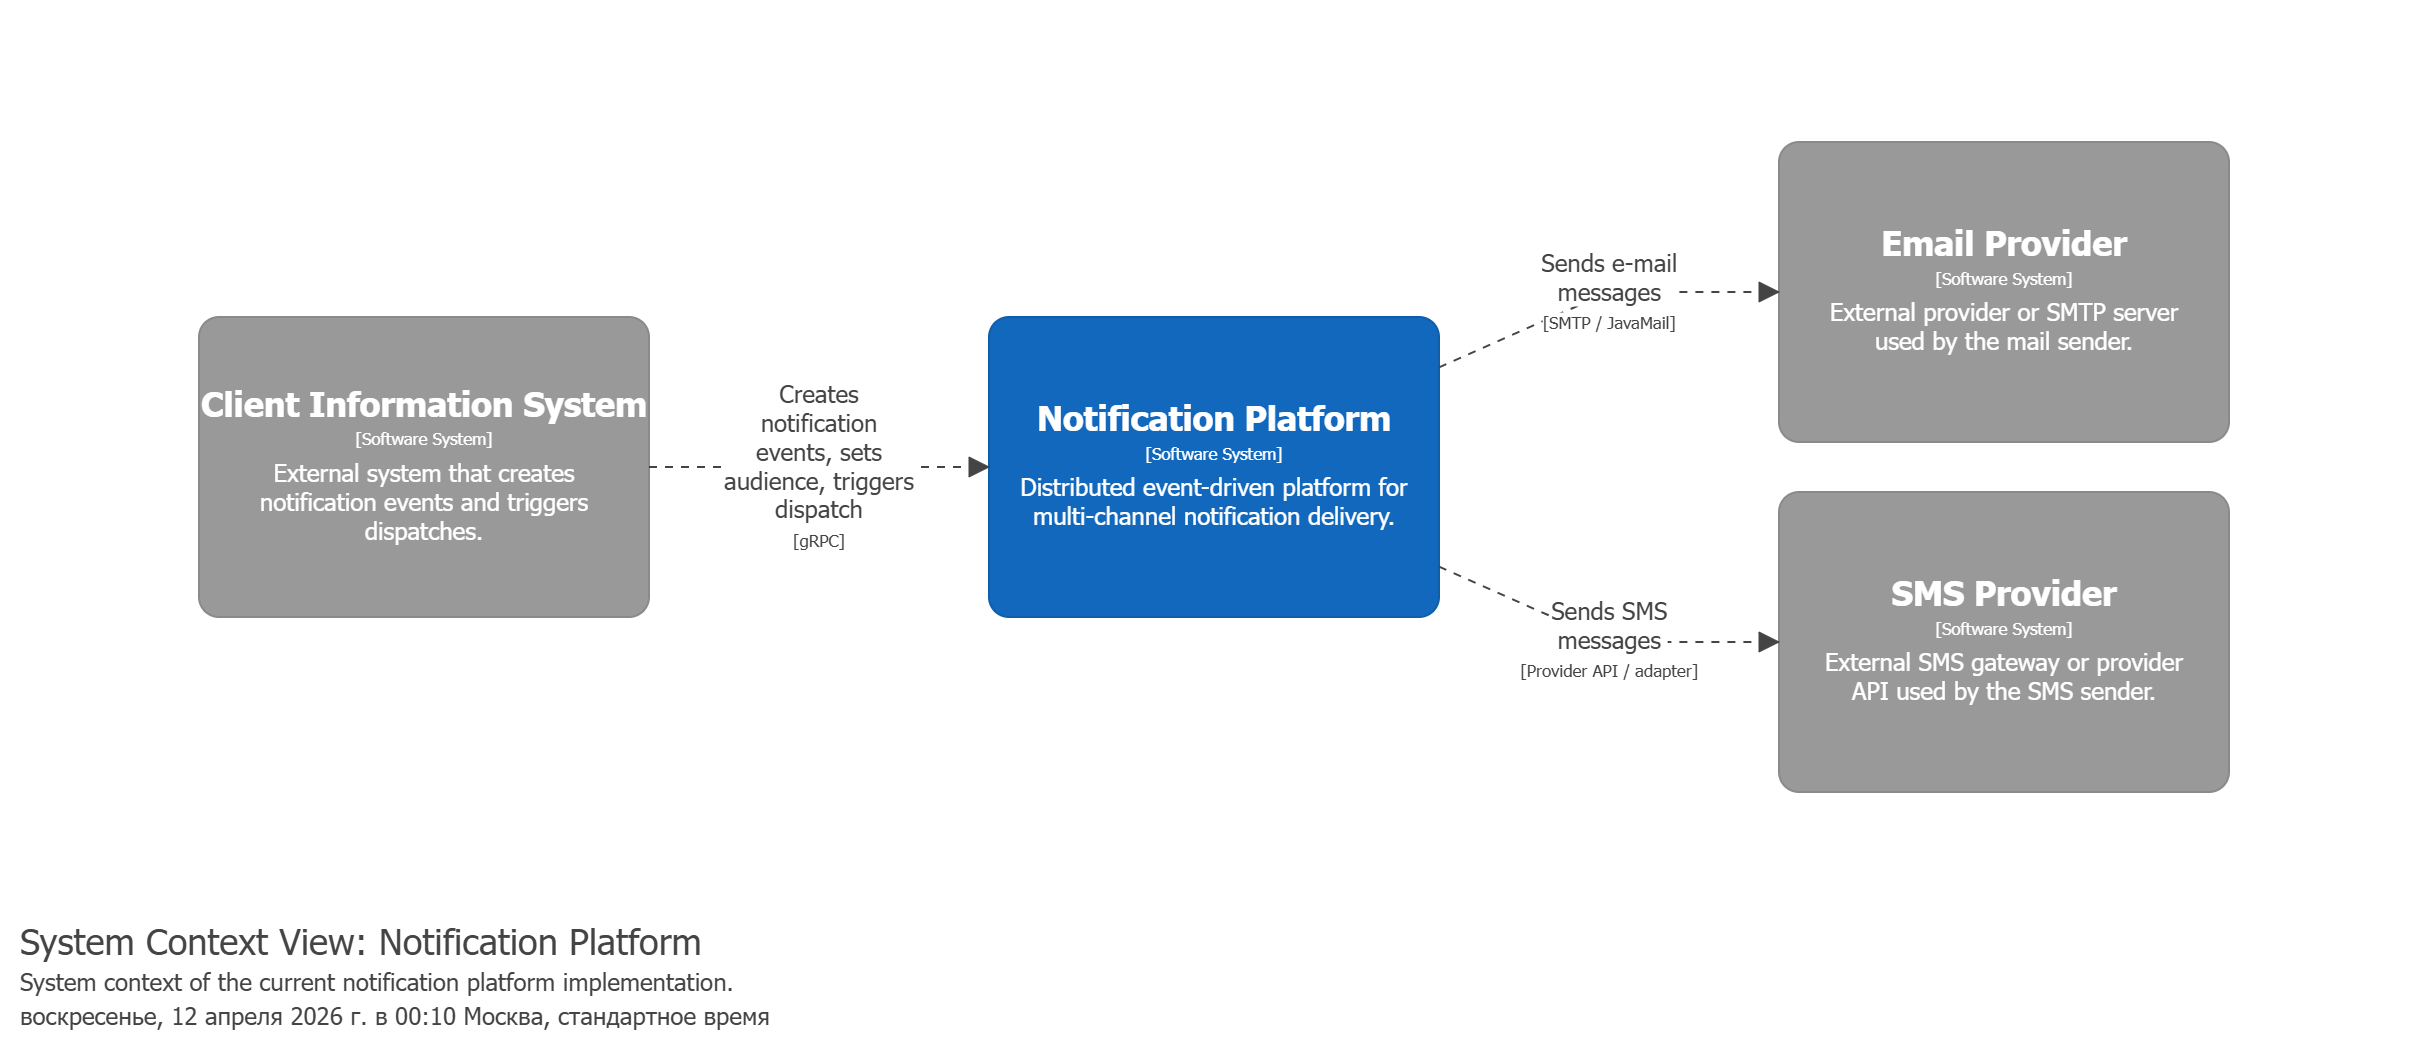
\includegraphics[width=\textwidth]{inc/structurizr-system-context.png}
    \caption{Системный контекст платформы уведомлений}
    \label{fig:arch-system-context-structurizr}
\end{figure}

Системный контекст нужен не как обзор компонентов, а как фиксация границы ответственности платформы. Клиентская система взаимодействует только с командным контуром, а внешние email- и SMS-провайдеры доступны только sender-сервисам. Это исключает прямую связность пользовательского запроса с внешним каналом связи и локализует риски деградации на стороне фоновой обработки.

\subsection{Контейнерная декомпозиция и границы ответственности}

Контейнерная декомпозиция определяется не только набором сервисов, но и владением данными. Каждый сервис, владеющий собственным состоянием, использует отдельное хранилище и не обращается напрямую к данным другого сервиса. Межсервисный обмен выполняется через gRPC и Kafka, а не через прямое чтение чужих таблиц или коллекций.

\begin{figure}[H]
    \centering
    \footnotesize
    \setlength{\tabcolsep}{4pt}
    \renewcommand{\arraystretch}{1.3}
    \begin{tabular}{ccc}
        \fbox{\parbox[c][1.6cm][c]{0.24\textwidth}{\centering Клиентская\\информационная система}} &
        $\rightarrow$ &
        \fbox{\parbox[c][1.6cm][c]{0.24\textwidth}{\centering Notification Facade\\gRPC-команды, аудитория, запуск доставки}} \\
        & & \fbox{\parbox[c][1.3cm][c]{0.24\textwidth}{\centering Facade PostgreSQL\\notification\_event, audience, dispatch, outbox}} \\[4pt]
        \fbox{\parbox[c][1.5cm][c]{0.24\textwidth}{\centering Template Registry\\версии шаблонов, предварительный рендеринг}} &
        \fbox{\parbox[c][1.5cm][c]{0.22\textwidth}{\centering Kafka\\notification.facade.events\\notification.mail.dispatches\\notification.mail.scheduled\\notification.sms.dispatches\\notification.delivery-statuses}} &
        \fbox{\parbox[c][1.5cm][c]{0.24\textwidth}{\centering Profile Consent\\проверка профиля получателя}} \\
        \fbox{\parbox[c][1.2cm][c]{0.24\textwidth}{\centering MongoDB Templates}} & &
        \fbox{\parbox[c][1.2cm][c]{0.24\textwidth}{\centering Redis Recipient Profiles}} \\[4pt]
        \fbox{\parbox[c][1.5cm][c]{0.24\textwidth}{\centering Scheduler Delivery\\отложенный запуск}} &
        \fbox{\parbox[c][1.5cm][c]{0.24\textwidth}{\centering Notification Mail Sender\\email-обработка, retry, status}} &
        \fbox{\parbox[c][1.5cm][c]{0.24\textwidth}{\centering Notification SMS Sender\\SMS-обработка, retry, status}} \\
        \fbox{\parbox[c][1.2cm][c]{0.24\textwidth}{\centering Scheduler PostgreSQL}} &
        \fbox{\parbox[c][1.2cm][c]{0.24\textwidth}{\centering Mail PostgreSQL}} &
        \fbox{\parbox[c][1.2cm][c]{0.24\textwidth}{\centering SMS PostgreSQL}} \\[4pt]
        \multicolumn{3}{c}{
            \fbox{\parbox[c][1.5cm][c]{0.30\textwidth}{\centering History Writer\\история статусов, сводки}}
            \hspace{0.02\textwidth}
            \fbox{\parbox[c][1.2cm][c]{0.20\textwidth}{\centering History PostgreSQL}}
        } \\[4pt]
        \multicolumn{3}{c}{
            \fbox{\parbox[c][1.1cm][c]{0.26\textwidth}{\centering Prometheus / Grafana}}
            \hspace{0.02\textwidth}
            \fbox{\parbox[c][1.1cm][c]{0.22\textwidth}{\centering SMTP /\\email-провайдер}}
            \hspace{0.02\textwidth}
            \fbox{\parbox[c][1.1cm][c]{0.22\textwidth}{\centering SMS-провайдер}}
        }
    \end{tabular}
    \caption{Контейнерная архитектура платформы уведомлений с разделением хранилищ по сервисным контурам}
    \label{fig:arch-containers-owned-storage}
\end{figure}

Рисунок~\ref{fig:arch-containers-owned-storage} отражает не только сервисы, но и владение данными. Notification Facade, Scheduler Delivery, Notification Mail Sender, Notification SMS Sender и History Writer используют отдельные PostgreSQL-хранилища. Template Registry владеет MongoDB-хранилищем шаблонов, а Profile Consent владеет Redis-хранилищем профилей получателей. Такое разделение исключает превращение базы данных в общий интеграционный слой и принуждает сервисы обмениваться данными только через контракт владельца.

\subsection{Верхнеуровневая модель данных и сервисных границ}

Архитектурная модель опирается на четыре уровня сущностей:
\begin{enumerate}
    \item уведомительное событие как описание намерения;
    \item запуск доставки как экземпляр исполнения события;
    \item канальная доставка как обработка пары «получатель --- канал»;
    \item история доставки как журнал и агрегированное представление итогов.
\end{enumerate}

Такое разделение определяет границы сервисов. Фасад владеет событием и запуском доставки, sender-сервисы владеют канальной доставкой и попытками отправки, history-writer владеет фактами изменения статуса. Template Registry и Profile Consent вынесены в отдельные контуры, поскольку они обслуживают сразу несколько этапов обработки и несколько каналов.

Состав контейнеров и их роль приведены в таблице~\ref{tab:architecture-containers}.

\begin{table}[H]
    \centering
    \footnotesize
    \renewcommand{\arraystretch}{1.15}
    \caption{Контейнеры и их ответственность}
    \label{tab:architecture-containers}
    \begin{tabular}{|L{0.24\textwidth}|L{0.38\textwidth}|L{0.25\textwidth}|}
        \hline
        \textbf{Контейнер} & \textbf{Ответственность} & \textbf{Собственное хранилище} \\
        \hline
        Notification Facade & Приём gRPC-команд, управление событиями, аудиторией и запусками доставки, публикация в Kafka. & Facade PostgreSQL \\
        \hline
        Template Registry & Хранение шаблонов, версий и канальных представлений, RenderPreview. & MongoDB Templates \\
        \hline
        Profile Consent & Выдача профиля получателя, разрешений каналов и адресных атрибутов. & Redis Recipient Profiles \\
        \hline
        Scheduler Delivery & Контур отложенной публикации запусков доставки. & Scheduler PostgreSQL \\
        \hline
        Notification Mail Sender & Обработка email-запусков, попытки отправки, retry и публикация статусов. & Mail PostgreSQL \\
        \hline
        Notification SMS Sender & Обработка SMS-запусков, попытки отправки, retry и публикация статусов. & SMS PostgreSQL \\
        \hline
        History Writer & Приём статусных событий, запись истории и формирование сводок. & History PostgreSQL \\
        \hline
        Kafka & Событийный обмен между сервисами и буферизация фоновой обработки. & Не применимо \\
        \hline
        Prometheus, Grafana & Наблюдаемость и контроль эксплуатационных показателей. & Метрики сервисов и Kafka-клиентов \\
        \hline
    \end{tabular}
\end{table}

\subsection{Верхнеуровневые потоки данных}

\subsubsection{Поток приёма команды и регистрации события}

Приём пользовательской команды выполняется в синхронном контуре. Notification Facade валидирует запрос, проверяет ключ идемпотентности, сохраняет уведомительное событие, аудиторию и запись outbox. Только после этого событие публикуется в Kafka для дальнейшей обработки.

Сценарий взаимодействий показан на рисунке~\ref{fig:arch-create-event-flow-structurizr}.

\begin{figure}[H]
    \centering
    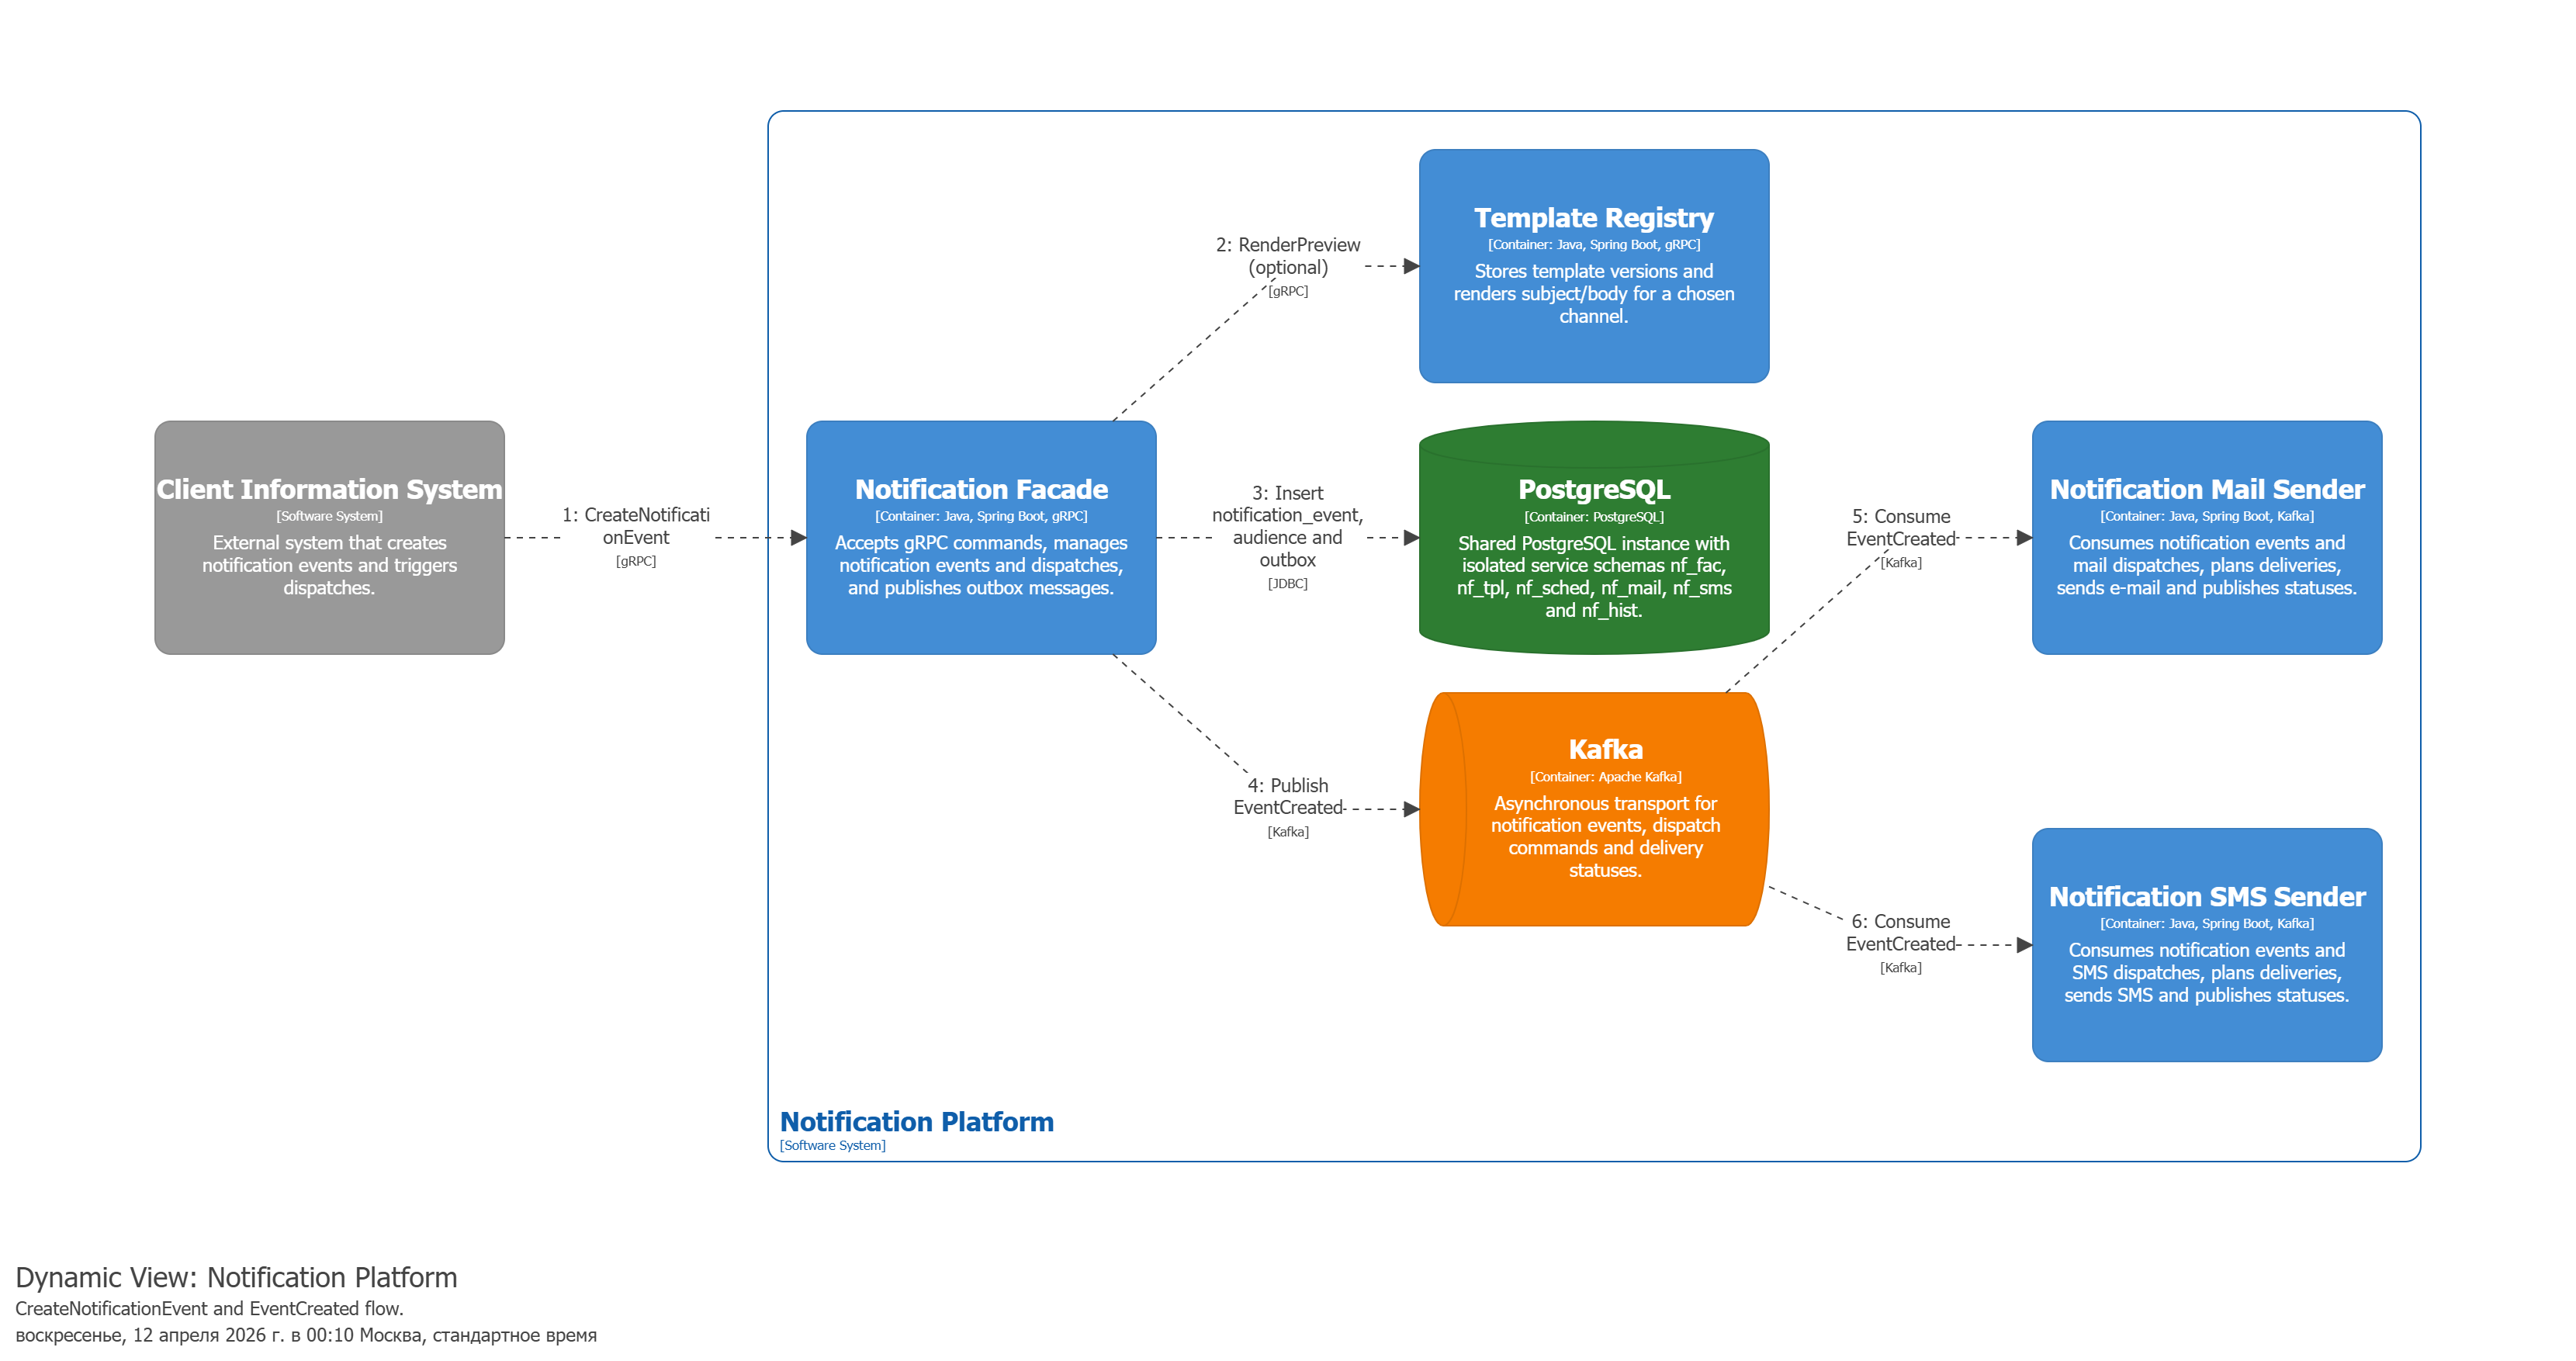
\includegraphics[width=\textwidth]{inc/structurizr-create-event-flow.png}
    \caption{Динамический поток регистрации события и передачи в событийный контур}
    \label{fig:arch-create-event-flow-structurizr}
\end{figure}

Рисунок~\ref{fig:arch-create-event-flow-structurizr} нужен для фиксации самой чувствительной точки архитектуры: перехода от синхронной команды к фоновому контуру. Именно здесь определяется, будет ли принятая команда потеряна при сбое сервиса между записью в базу и публикацией в брокер. В выбранной архитектуре этот риск закрывается локальной транзакцией и transactional outbox.

\subsubsection{Поток запуска доставки}

Запуск доставки отделён от этапа приёма команды. Такое решение даёт три практических эффекта:
\begin{enumerate}
    \item запуск можно выполнить сразу или по расписанию без изменения самой модели события;
    \item повторный запуск допустим без пересоздания уведомительного события;
    \item сбой канального контура не влияет на уже завершённый клиентский запрос.
\end{enumerate}

\subsubsection{Поток отложенной доставки}

Отложенная доставка вынесена в самостоятельный контур Scheduler Delivery. Фасад публикует запуск в отдельный scheduled-топик, планировщик сохраняет задачу в собственном PostgreSQL-хранилище и после наступления планового времени переводит её в рабочий Kafka-топик. Хранение отложенных задач в отдельном сервисе исключает зависимость от таймеров в памяти конкретного экземпляра приложения.

\subsubsection{Поток канальной обработки и истории}

Mail Sender и SMS Sender потребляют свои рабочие топики независимо друг от друга. Перед фактической отправкой sender-сервис обращается к profile-consent, получает решение по получателю и либо выполняет отправку, либо фиксирует пропуск как доменный результат обработки. После завершения попытки sender публикует статусное событие, которое history-writer записывает в собственное хранилище и агрегирует для запросов чтения.

\subsection{Kafka-архитектура событийного контура}

Kafka используется как базовый транспорт асинхронного обмена между контурами:
\begin{enumerate}
    \item поток событий жизненного цикла уведомления;
    \item потоки рабочих запусков по каналам;
    \item поток отложенных email-запусков;
    \item поток статусных событий доставки.
\end{enumerate}

Ключевые топики текущей архитектуры приведены в таблице~\ref{tab:kafka-architecture-topics}.

\begin{table}[h]
    \centering
    \footnotesize
    \renewcommand{\arraystretch}{1.15}
    \caption{Kafka-топики и их назначение}
    \label{tab:kafka-architecture-topics}
    \begin{tabular}{|L{0.34\textwidth}|L{0.52\textwidth}|}
        \hline
        \textbf{Топик} & \textbf{Назначение} \\
        \hline
        \seqsplit{notification.facade.events} & События жизненного цикла уведомления, публикуемые фасадом для дальнейшей канальной обработки. \\
        \hline
        \seqsplit{notification.mail.dispatches} & Рабочие команды на email-доставку. \\
        \hline
        \seqsplit{notification.mail.scheduled} & Отложенные email-команды, которые сначала обрабатывает Scheduler Delivery. \\
        \hline
        \seqsplit{notification.sms.dispatches} & Рабочие команды на SMS-доставку. \\
        \hline
        \seqsplit{notification.delivery-statuses} & Итоговые статусы email- и SMS-доставки, поступающие в history-writer. \\
        \hline
    \end{tabular}
\end{table}

Таблица~\ref{tab:kafka-architecture-topics} показывает, что Kafka используется не как внешний интеграционный шлюз, а как внутренний транспорт для нескольких независимых стадий обработки. Отдельные рабочие топики по каналам позволяют масштабировать sender-сервисы независимо и не смешивать email- и SMS-обработку в одном consumer-контуре.

\subsubsection{Маршрут событийного потока}

Маршрут обработки в Kafka-контуре может быть представлен как последовательность доменных шагов:
\begin{enumerate}
    \item фасад публикует событие жизненного цикла уведомления в notification.facade.events;
    \item фасад формирует каналоспецифичный запуск и публикует его в notification.mail.dispatches или notification.sms.dispatches;
    \item при отложенной отправке запуск сначала попадает в notification.mail.scheduled, затем планировщик переносит его в рабочий топик;
    \item канальные обработчики публикуют итог в notification.delivery-statuses;
    \item сервис истории консолидирует статусные события в агрегированное представление получателя.
\end{enumerate}

\subsection{Механизмы надёжности на архитектурном уровне}

Надёжность обеспечивается сочетанием архитектурных механизмов:
\begin{enumerate}
    \item transactional outbox в фасаде и sender-сервисах для согласования доменного изменения и публикации интеграционного сообщения;
    \item transactional inbox в канальных обработчиках для регистрации входящего Kafka-сообщения перед бизнес-обработкой;
    \item idempotency key и уникальные ограничения для повторных команд и повторной доставки сообщения брокером;
    \item retry для временных ошибок и статусная модель для окончательных ошибок;
    \item history-writer как контур накопления фактов изменения статуса.
\end{enumerate}

Эта схема соответствует модели at-least-once доставки и управляемой eventual consistency между сервисами \cite{kafka_docs,richardson_patterns}. Дубликаты в транспортном слое допускаются, но подавляются на уровне приложения ключами идемпотентности, входящими журналами и уникальными ограничениями.

\subsection{Архитектура профиля получателя}

Профиль получателя выделен в отдельный сервисный контур. Profile Consent является единственной точкой доступа к Redis-хранилищу профилей получателей. Канальные сервисы не обращаются к Redis напрямую, а получают решение о допустимости доставки через сервисный контракт profile-consent.

На архитектурном уровне профиль включает:
\begin{enumerate}
    \item активность получателя;
    \item разрешения и ограничения по каналам;
    \item адресные данные, необходимые для email и SMS;
    \item технические атрибуты актуальности профиля.
\end{enumerate}

\subsection{Архитектура шаблонного контура}

Template Registry является единственным владельцем MongoDB-хранилища шаблонов. Остальные сервисы не обращаются к MongoDB напрямую и получают шаблонное содержимое только через сервисный контракт template-registry.

Выбор документоориентированной модели обусловлен структурой предметной сущности. Шаблон включает метаданные, активную версию и несколько канальных представлений, которые в типовом сценарии читаются совместно. Хранение этих данных в одном документе уменьшает число операций чтения при RenderPreview и при выборе активной версии для отправки \cite{mongodb_docs}.

\subsection{Архитектура наблюдаемости}

Наблюдаемость проектируется как обязательная часть архитектуры. Каждый сервис экспортирует метрики, достаточные для восстановления маршрута от входной команды до записи статуса в историю. Наиболее значимыми для этой платформы являются четыре группы метрик:
\begin{enumerate}
    \item gRPC server metrics командного контура;
    \item Kafka producer metrics на публикации событий и статусных сообщений;
    \item Kafka listener metrics на канальной обработке и в history-writer;
    \item JVM и process metrics для оценки ресурсных ограничений.
\end{enumerate}

Такой набор нужен не для общего мониторинга инфраструктуры, а для диагностики разрыва маршрута обработки: принят ли запрос, опубликовано ли событие, дошло ли оно до sender-сервиса и записан ли итоговый статус \cite{spring_boot_docs,kafka_docs}.

\subsection{Безопасность}

В пределах работы безопасность рассматривается на уровне сервисных границ и владения данными. Прикладной сервис не читает чужое хранилище напрямую, а использует только контракт владельца. Это уменьшает площадь непреднамеренного воздействия, упрощает разграничение ответственности и исключает зависимость бизнес-логики от внутренней схемы чужого хранилища.

Выбранная архитектура задаёт основу реализации: gRPC используется для командного контура, Kafka --- для фоновой обработки, а сохранность и повторяемость обработки обеспечиваются outbox/inbox, идемпотентностью и историей статусов.

    \section{Реализация системы}

Реализация выполнена как набор сервисов на Java~25 и Spring Boot. Код размещён в Gradle monorepo: прикладные сервисы, protobuf-контракты и вспомогательные библиотеки собираются независимо, но используют единый набор соглашений по конфигурации, наблюдаемости и интеграции.

Взаимодействие синхронных контуров построено на gRPC. Асинхронная обработка команд доставки, статусов и fallback-событий выполняется через Kafka. Для транзакционных данных используются PostgreSQL-хранилища, для шаблонов --- MongoDB, для истории статусов --- ClickHouse. Redis используется только для TTL-механизмов: отметок отмены и локального подавления дублей в sender-сервисах.

\subsection{Обзор владения данными}

Хранилища разделены по сервисным границам. Сервис не читает таблицы или коллекции другого сервиса напрямую: доступ к данным выполняется через gRPC-контракт или через события Kafka. Такое разделение снижает связность схем данных и не превращает базу данных в общий интеграционный слой.

\begin{table}[h]
    \centering
    \footnotesize
    \renewcommand{\arraystretch}{1.15}
    \caption{Владение данными по сервисным контурам}
    \label{tab:data-ownership}
    \begin{tabular}{|L{0.22\textwidth}|L{0.18\textwidth}|L{0.36\textwidth}|L{0.16\textwidth}|}
        \hline
        \textbf{Сервис} & \textbf{Хранилище} & \textbf{Данные} & \textbf{Доступ других сервисов} \\
        \hline
        Notification Facade & Facade PostgreSQL & События уведомлений, аудитория, входные dispatch-запросы, outbox-записи и ключи идемпотентности. & Только через gRPC/Kafka \\
        \hline
        Template Registry & MongoDB Templates & Шаблоны, версии шаблонов, channel contents и activeVersion. & Через gRPC \\
        \hline
        Profile Consent & Profile Consent PostgreSQL & Профиль получателя, tenant-aware разрешения каналов, destination и ограничения. & Через gRPC \\
        \hline
        Delivery Dispatcher & Dispatcher PostgreSQL & Отложенные задачи, routing decisions, retry/fallback state и состояние планирования. & Через Kafka/gRPC \\
        \hline
        Cancellation Service & Redis Cancellation Marks & Отметки отмены dispatch/delivery с TTL 30 минут. & Через gRPC \\
        \hline
        Notification Mail Sender & Redis Mail Dedup & TTL-ключи локального dedup для email-команд. & Не используется другими сервисами \\
        \hline
        Notification SMS Sender & Redis SMS Dedup & TTL-ключи локального dedup для SMS-команд. & Не используется другими сервисами \\
        \hline
        History Writer & ClickHouse History Store & Append-only история статусов доставки и атрибуты обработки. & Через API history-writer \\
        \hline
    \end{tabular}
\end{table}

DBML-версии реляционных схем подготовлены отдельно в каталоге docs/dbdiagram. Они используются как источник для ERD-изображений в данном разделе; PlantUML-версии схем сохранены в каталоге docs/plantuml.

\subsection{notification-facade}

Notification Facade принимает клиентские команды, проверяет входные данные, фиксирует событие уведомления и аудиторию, подготавливает dispatch request и публикует его в Kafka topic delivery.dispatcher. В этом сервисе остаются операции, связанные с входным жизненным циклом события: идемпотентность клиентской команды, запись события, работа с аудиторией и формирование outbox-записей для последующей публикации.

Фасад не отправляет команды напрямую в mail- или sms-sender. После подготовки события он публикует общий dispatch request, а выбор канала и fallback-решения выполняет delivery-dispatcher. При клиентской отмене фасад вызывает cancellation-service и не хранит отметки отмены в собственной PostgreSQL-схеме.

Основные таблицы фасада отражают входное событие, адресатов, dispatch-запрос и outbox. Реляционная модель приведена на рисунке~\ref{fig:data-facade-postgres-schema}.

\begin{figure}[H]
    \centering
    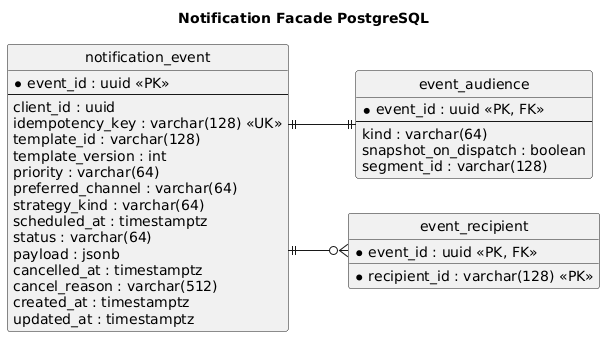
\includegraphics[width=0.82\textwidth]{inc/dbdiagram/png/facade-postgres-schema.png}
    \caption{Реляционная модель notification-facade}
    \label{fig:data-facade-postgres-schema}
\end{figure}

\subsection{template-registry}

Template Registry отвечает за хранение и рендеринг шаблонов уведомлений. Сервис получает от фасада идентификатор шаблона, канал и параметры рендеринга, выбирает активную версию и возвращает подготовленное содержимое. Модель хранится в MongoDB, потому что документ шаблона содержит версии, канальные представления и набор переменных, которые удобнее хранить как вложенную структуру.

В документе шаблона фиксируются client id, template id, activeVersion и набор версий. Для каждой версии хранятся channel contents для email и SMS, тема, тело и metadata. Пример структуры документа показан на рисунке~\ref{fig:data-template-registry-mongo}.

\begin{figure}[H]
    \centering
    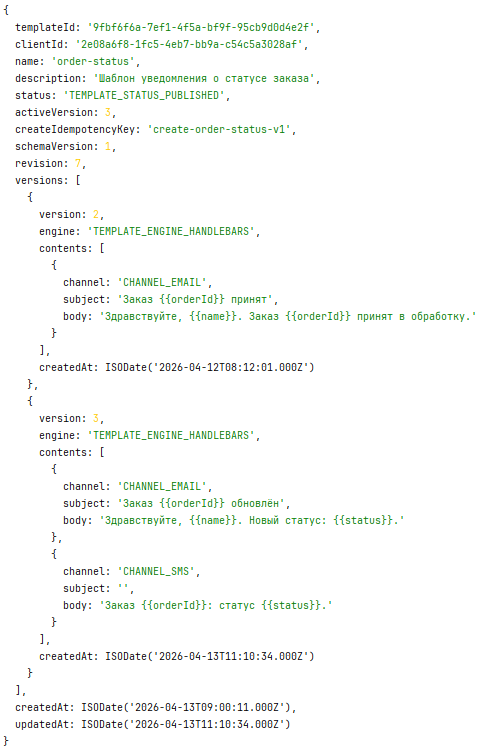
\includegraphics[width=0.76\textwidth]{inc/mongo-template-data.png}
    \caption{Модель MongoDB-документа template-registry}
    \label{fig:data-template-registry-mongo}
\end{figure}

\subsection{profile-consent}

Profile Consent инкапсулирует правила доступности каналов и профиль получателя. Delivery Dispatcher и другие сервисы не обращаются к таблицам профиля напрямую: они используют gRPC-метод проверки канала. Это сохраняет единое место принятия решений по recipient/channel/tenant.

PostgreSQL используется как транзакционное хранилище долговременных настроек профиля, согласий, channel destination и признаков блокировки. Основная таблица фиксирует активность профиля и предпочтительный канал, а таблица согласий хранит пару channel-tenant, destination, признак enabled и блокировку. Реляционная модель profile-consent приведена на рисунке~\ref{fig:data-profile-consent-postgres-schema}.

\begin{figure}[H]
    \centering
    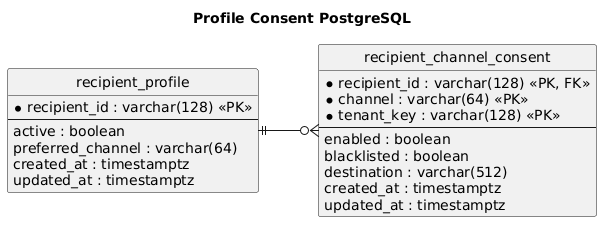
\includegraphics[width=0.82\textwidth]{inc/dbdiagram/png/profile-consent-postgres-schema.png}
    \caption{Реляционная модель profile-consent}
    \label{fig:data-profile-consent-postgres-schema}
\end{figure}

\subsection{delivery-dispatcher}

Delivery Dispatcher потребляет dispatch requests из delivery.dispatcher и fallback events из delivery.fallback. Сервис управляет отложенным запуском, принимает routing-решение, проверяет профиль и согласия через profile-consent, публикует команды в канальные Kafka topics и защищает fallback от бесконечного цикла.

Dispatcher не выполняет входную бизнес-валидацию, не работает с аудиторией и не рендерит шаблоны. Эти операции остаются в notification-facade. Его зона ответственности начинается после появления валидного dispatch request в Kafka и ограничена оркестрацией доставки, планированием и маршрутизацией.

Собственная PostgreSQL-модель dispatcher хранит планировочное состояние, routing decisions, retry/fallback state и технические данные, которые нужны для безопасного повторного запуска. Схема показана на рисунке~\ref{fig:data-dispatcher-postgres-schema}.

\begin{figure}[H]
    \centering
    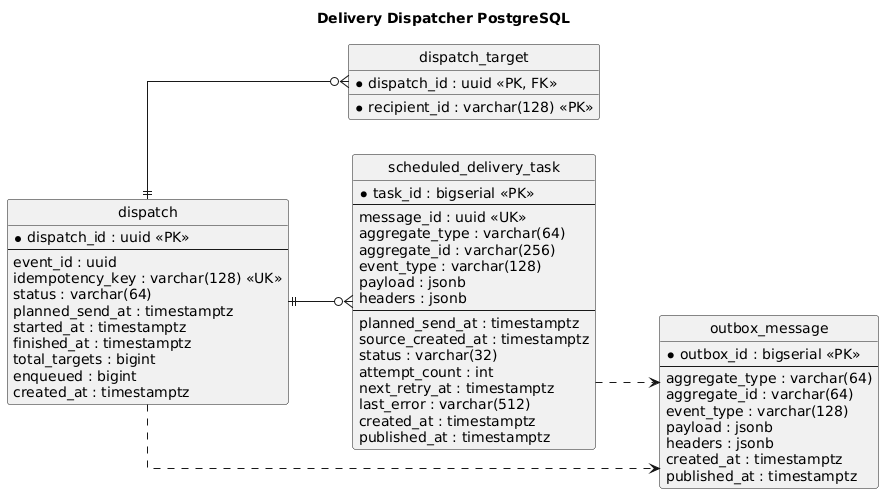
\includegraphics[width=0.86\textwidth]{inc/dbdiagram/png/dispatcher-postgres-schema.png}
    \caption{Реляционная модель delivery-dispatcher}
    \label{fig:data-dispatcher-postgres-schema}
\end{figure}

\subsection{cancellation-service}

Cancellation Service выделен в отдельный контур, потому что отмена dispatch/delivery должна быстро проверяться sender-сервисами перед обращением к внешнему провайдеру. Сервис предоставляет gRPC-методы фиксации отмены и проверки допустимости отправки.

Отметка отмены хранится в Redis как TTL-key. Время жизни ключа составляет 30 минут: после этого окно практической отмены считается закрытым, а дальнейшая судьба доставки определяется обычным статусным контуром. Повторный запрос отмены обрабатывается идемпотентно. Если sender получает признак отмены, он не вызывает внешний provider API и публикует статус CANCELED.

\subsection{notification-mail-sender}

Notification Mail Sender потребляет email-команды из Kafka и выполняет только execution-level проверки. Перед отправкой сервис атомарно записывает Redis dedup key через операцию типа SET NX EX, затем обращается к cancellation-service. Если доставка отменена, внешний email provider не вызывается, а в Kafka публикуется статус CANCELED.

Если отмены нет, sender выполняет отправку через SMTP/provider API и публикует итоговый статус. При окончательной ошибке email-канала сервис не выбирает альтернативный канал самостоятельно. Он публикует fallback event в delivery.fallback, после чего решение принимает delivery-dispatcher.

\subsection{notification-sms-sender}

Notification SMS Sender устроен аналогично mail sender. Он потребляет SMS-команды, выполняет локальный Redis-based dedup, проверяет cancellation-service и только после этого вызывает SMS provider API. При отмене публикуется статус CANCELED; при технической ошибке фиксируется статус доставки через общий Kafka status pipeline.

SMS sender не владеет шаблонами, профилем получателя или правилами fallback. Эти решения остаются в template-registry, profile-consent и delivery-dispatcher соответственно.

\subsection{history-writer}

History Writer вынесен из online-path доставки и работает как потребитель status events из Kafka. Сервис записывает события статусов в ClickHouse в append-only модель. Такая схема позволяет отделить аналитическое чтение истории от транзакционных контуров notification-facade и delivery-dispatcher.

ClickHouse-таблица содержит идентификаторы события, dispatch и delivery, канал, статус, причину ошибки, номер попытки, время возникновения статуса и технические атрибуты Kafka-публикации. Модель хранения истории приведена на рисунке~\ref{fig:data-history-clickhouse-schema}.

\begin{figure}[H]
    \centering
    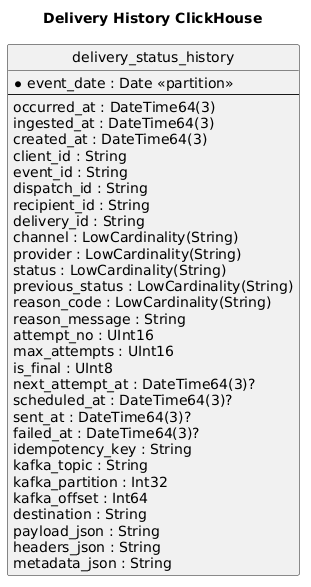
\includegraphics[width=0.38\textwidth]{inc/dbdiagram/png/history-clickhouse-schema.png}
    \caption{Модель хранения истории доставки в ClickHouse}
    \label{fig:data-history-clickhouse-schema}
\end{figure}

    \section{Развёртывание, эксплуатация и экспериментальная проверка}

\subsection{Стенд и контур проверки}

Экспериментальная проверка выполнялась на контейнерном стенде, разворачиваемом через Docker Compose. В состав стенда входили прикладные сервисы notification-facade, template-registry, profile-consent, scheduler-delivery, notification-mail-sender, notification-sms-sender и history-writer, а также Kafka, отдельные PostgreSQL-хранилища операционных сервисов, MongoDB, Redis, ClickHouse, Prometheus и Grafana.

Такой стенд воспроизводит не только набор сервисов, но и границы хранения, поэтому подходит для проверки маршрута целиком: gRPC-команда, запись события, Kafka-публикация, sender-обработка и запись результата в аналитическую историю доставки.

Стенд запускался локально на рабочей станции под управлением Windows 10 с процессором класса Intel Core i7 13-го поколения и 16~ГБ оперативной памяти. Это важно для интерпретации результатов: проверка проводилась не на выделенном сервере, а в ограниченном локальном окружении, где контейнеры приложений, брокер, базы данных и средства наблюдаемости конкурировали за одни и те же ресурсы хоста.

Ключевые параметры нагрузочного стенда и генератора приведены в таблице~\ref{tab:load-stand-config}. В основной части оставлены только те настройки, которые влияют на интерпретацию маршрута и масштаба нагрузки.

\begin{table}[H]
    \centering
    \footnotesize
    \renewcommand{\arraystretch}{1.15}
    \caption{Конфигурация нагрузочного стенда}
    \label{tab:load-stand-config}
    \begin{tabular}{|L{0.34\textwidth}|L{0.50\textwidth}|}
        \hline
        \textbf{Параметр} & \textbf{Значение} \\
        \hline
        Платформа хоста & Windows 10, локальный запуск в Docker Compose \\
        \hline
        Аппаратная конфигурация & процессор класса Intel Core i7 13-го поколения, 16 ГБ RAM \\
        \hline
        Число уникальных пользователей & 10000 подготовленных получателей \\
        \hline
        Число потоков генератора & 10 \\
        \hline
        Профиль входной нагрузки & линейный разгон от 25 до 90 запросов в секунду \\
        \hline
        Длительность активной фазы & 1800 секунд \\
        \hline
        Получателей в одном запросе & случайное число от 2 до 10 \\
        \hline
    \end{tabular}
\end{table}

\subsection{Методика проверки}

Нагрузочный прогон использовался для двух задач: проверки связности полного маршрута обработки и получения базовых количественных характеристик стенда. Целью не было определение предельной промышленной производительности, однако полученные значения RPS и задержек позволяют оценить поведение системы под устойчивой нагрузкой.

Проверка выполнялась в четыре этапа:
\begin{enumerate}
    \item подготовка стенда и приведение хранилищ к контролируемому начальному состоянию;
    \item выполнение функциональных и сквозных сценариев;
    \item серия из трёх повторных нагрузочных прогонов через custom-loader после предварительного заполнения Redis-профилей;
    \item сбор и интерпретация метрик gRPC, Kafka и JVM по артефактам Grafana.
\end{enumerate}

До серии нагрузочных прогонов выполнялись подготовительный seed получателей и ручная проверка базовых сценариев: создание события, немедленный запуск, отложенный запуск, email-доставка, SMS-доставка и запись итогового статуса в history-writer. Повторные прогоны выполнялись с одним и тем же профилем нагрузки; в тексте ниже приводятся усреднённые значения и характерные диапазоны порядка величин, а не псевдоточные цифры до единиц сообщений.

\subsection{Критерии успешности}

Критерии успешности нагрузочного прогона приведены в таблице~\ref{tab:test-success-criteria}.

\begin{table}[H]
    \centering
    \footnotesize
    \renewcommand{\arraystretch}{1.15}
    \caption{Критерии успешности нагрузочного прогона}
    \label{tab:test-success-criteria}
    \begin{tabular}{|L{0.27\textwidth}|L{0.29\textwidth}|L{0.30\textwidth}|}
        \hline
        \textbf{Критерий} & \textbf{Ожидаемый результат} & \textbf{Фактический результат} \\
        \hline
        Входной gRPC-контур принимает команды & Метрика CreateNotificationEvent имеет ненулевой поток запросов в активной фазе & Ненулевой поток подтверждён графиком server RPS; медианная задержка CreateNotificationEvent составила около 786 ms \\
        \hline
        События передаются в Kafka & Producer и listener metrics фиксируют публикацию и потребление сообщений & Для notification.facade.events среднее потребление составило 38.3 сообщения в секунду, максимум 47.3 сообщения в секунду \\
        \hline
        Sender-сервисы потребляют события & Канальные listener-метрики имеют ненулевой поток и конечное время обработки & Среднее listener-время mail-sender составило 47.2 ms, для scheduler-delivery --- 41--58 ms в сценарии отложенного запуска \\
        \hline
        Статусы доходят до history-writer & delivery-statuses потребляются и сохраняются & Среднее потребление notification.delivery-statuses составило 21.5 сообщения в секунду, среднее listener-время history-writer --- 46.9 ms \\
        \hline
        Система остаётся наблюдаемой & Доступны gRPC, Kafka и JVM-метрики по всем ключевым участкам маршрута & Маршрут восстанавливается по Grafana-артефактам server RPS, gRPC latency, Kafka publish latency и Kafka consume RPS \\
        \hline
    \end{tabular}
\end{table}

\subsection{Проверка механизмов повторной обработки}

Таблица~\ref{tab:repeat-processing-checks} отделяет заявленные механизмы repeat-processing от общей нагрузки и показывает, какие сценарии были подтверждены на стенде, а какие требуют отдельной дополнительной фиксации.

\begin{table}[H]
    \centering
    \footnotesize
    \renewcommand{\arraystretch}{1.15}
    \caption{Проверка механизмов повторной обработки}
    \label{tab:repeat-processing-checks}
    \begin{tabular}{|L{0.26\textwidth}|L{0.19\textwidth}|L{0.22\textwidth}|L{0.23\textwidth}|}
        \hline
        \textbf{Сценарий} & \textbf{Проверяемый механизм} & \textbf{Ожидаемый результат} & \textbf{Фактический результат} \\
        \hline
        Повторный CreateNotificationEvent с тем же idempotency key & idempotency key, unique constraint & Новое уведомительное событие не создаётся & TODO: требуется зафиксировать отдельный протокол повторного вызова и ответ фасада в артефактах стенда \\
        \hline
        Повторное получение Kafka-сообщения sender-сервисом & transactional inbox, deduplication & Доставка не создаётся повторно & Сценарий заложен в модель consumer inbox и уникальных ограничений; в текущем наборе выгрузок отдельный счётчик подавленных дублей отсутствует \\
        \hline
        Временная ошибка внешнего провайдера & retry policy & Доставка переводится в повторную попытку или в контролируемую ошибку & TODO: требуется сохранить отдельный лог или метрику по retry для mail- и sms-контуров \\
        \hline
        Недоступность profile-consent при канальной обработке & ошибка профильной проверки, статусная фиксация & Сообщение не теряется; результат фиксируется статусом или повторной попыткой & Проверен отказозависимый маршрут через обязательный вызов profile-consent; отдельная статистика по forced-failure в текущем прогоне не сохранялась \\
        \hline
        Запись итогового статуса в history-writer & status event, Kafka, history storage & Изменение статуса появляется в истории & Подтверждено потреблением notification.delivery-statuses и записью итогового статуса в history-writer \\
        \hline
    \end{tabular}
\end{table}

\subsection{Проверенные сценарии}

На стенде были подтверждены следующие сценарии:
\begin{enumerate}
    \item создание уведомительного события и фиксация аудитории;
    \item немедленный запуск доставки;
    \item отложенный запуск через scheduler-delivery;
    \item обработка email- и SMS-запусков как двух независимых канальных контуров;
    \item проверка профиля получателя перед отправкой;
    \item запись итогового статуса в history-writer;
    \item повторная обработка входящего сообщения без неконтролируемого дубля.
\end{enumerate}

Функциональная проверка показала, что полный маршрут не распадается на несвязанные фрагменты: событие, запуск, канальная доставка и история проходят через разные сервисные границы, но сохраняют идентифицируемую связь.

\subsection{Артефакты метрик}

Для анализа использовались четыре группы метрик:
\begin{enumerate}
    \item gRPC server metrics для notification-facade, profile-consent и history-writer;
    \item Kafka producer metrics для публикации событий и статусных сообщений;
    \item Kafka listener metrics для sender-сервисов и history-writer;
    \item JVM/process metrics как эксплуатационный фон.
\end{enumerate}

\begin{figure}[H]
    \centering
    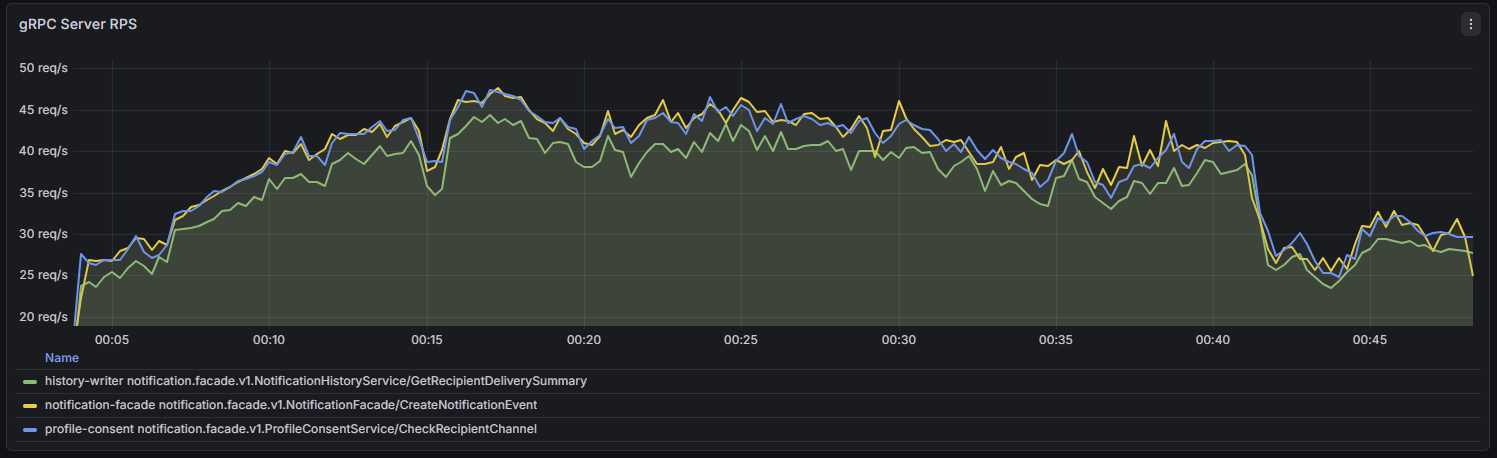
\includegraphics[width=\textwidth]{inc/server_rps.png}
    \caption{Интенсивность gRPC-вызовов в ходе нагрузочного прогона}
    \label{fig:test-server-rps}
\end{figure}

Рисунок~\ref{fig:test-server-rps} используется как временная шкала активной фазы прогона. По нему видно, что CreateNotificationEvent, CheckRecipientChannel и GetRecipientDeliverySummary наблюдаются как независимые сервисные вызовы, а не как один монолитный маршрут. Для архитектуры это подтверждает разделение ролей между фасадом, profile-consent и history-writer.

\begin{figure}[H]
    \centering
    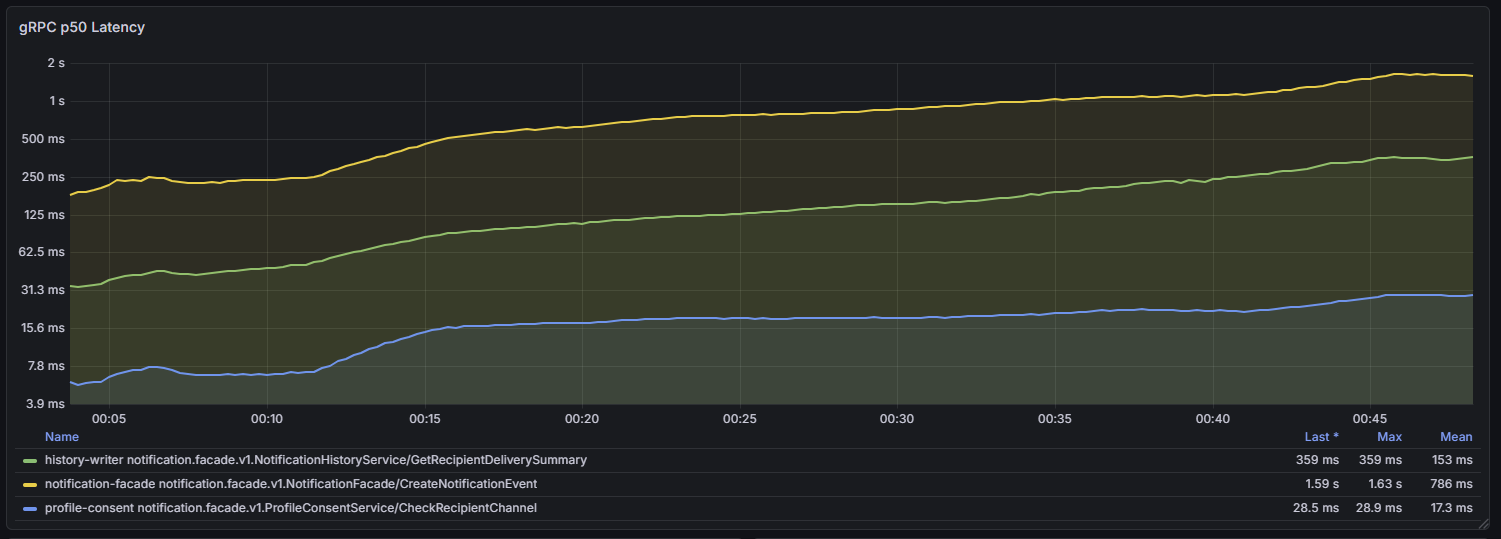
\includegraphics[width=\textwidth]{inc/grpc_p50_lat.png}
    \caption{Медианная задержка gRPC-вызовов}
    \label{fig:test-grpc-p50}
\end{figure}

Рисунок~\ref{fig:test-grpc-p50} показывает, что самый тяжёлый синхронный вызов в наблюдаемом наборе --- CreateNotificationEvent. Это ожидаемо: именно на этом этапе выполняются валидация запроса, запись события и подготовка публикации в Kafka. При этом задержки profile-consent и history-writer остаются существенно ниже, что подтверждает их роль как поддерживающих сервисов, а не доминирующих узких мест командного контура.

\begin{figure}[H]
    \centering
    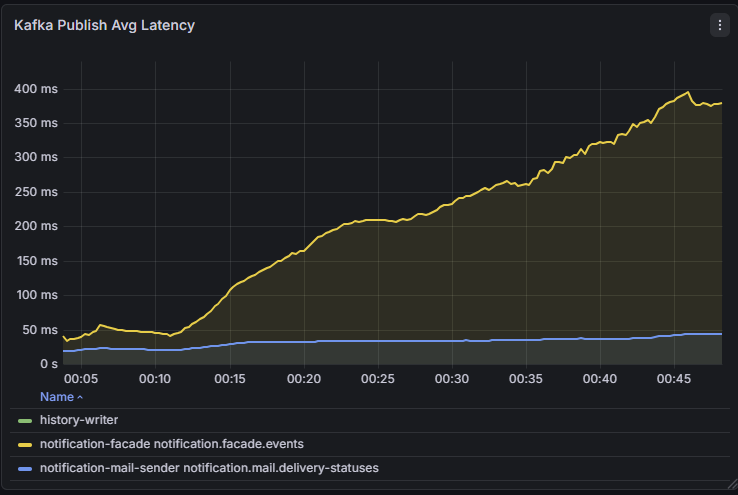
\includegraphics[width=\textwidth]{inc/kafka_avg_latency.png}
    \caption{Средняя задержка публикации Kafka-сообщений}
    \label{fig:test-kafka-publish-latency}
\end{figure}

Рисунок~\ref{fig:test-kafka-publish-latency} нужен для оценки стоимости перехода из синхронного контура в асинхронный. Рост средней задержки публикации для notification.facade.events показывает, что брокер и producer-участок дают заметный вклад в суммарное время маршрута. Одновременно график остаётся ограниченным сверху и не показывает признаков необратимого накопления деградации.

\begin{figure}[H]
    \centering
    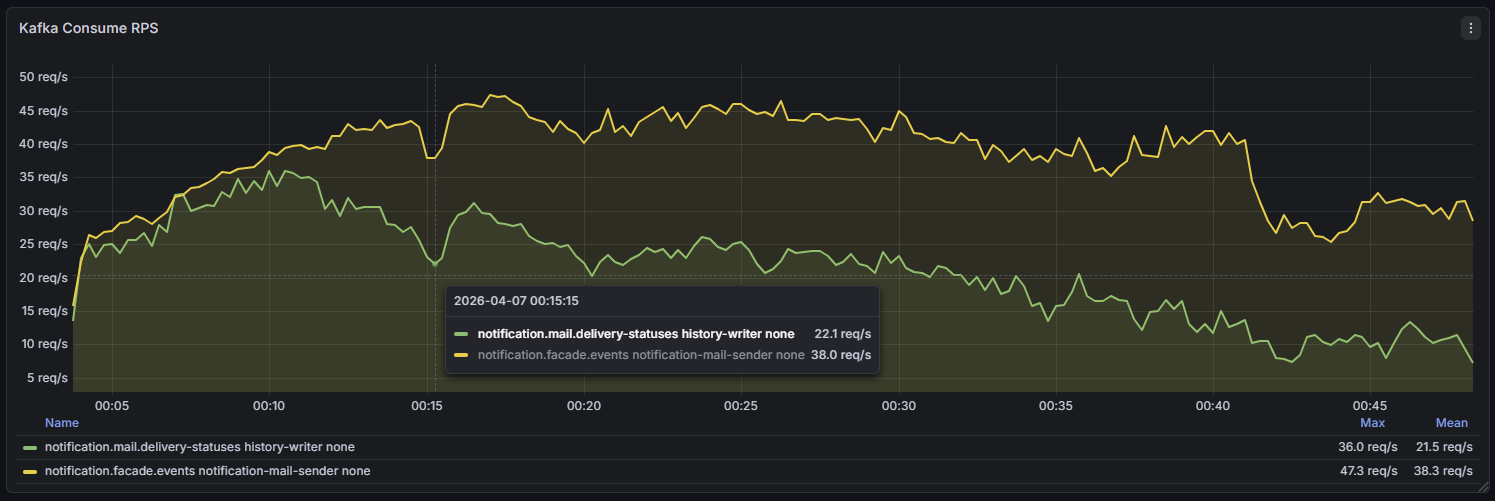
\includegraphics[width=\textwidth]{inc/kafka_consume_rps.png}
    \caption{Интенсивность потребления Kafka-сообщений}
    \label{fig:test-kafka-consume-rps}
\end{figure}

Рисунок~\ref{fig:test-kafka-consume-rps} подтверждает прохождение маршрута до конечной стадии. На нём одновременно видны потребление notification.facade.events канальным обработчиком и потребление notification.delivery-statuses сервисом history-writer. Это означает, что нагрузочный прогон затрагивает не только входной фасад и публикацию в Kafka, но и завершение жизненного цикла уведомления.

\subsection{Результаты нагрузочного прогона}

Итоговые показатели серии прогонов приведены в таблицах~\ref{tab:load-results-volume} и~\ref{tab:load-results-latency}. Числа даны как усреднённые ориентиры и диапазоны по трём повторным прогонам с одинаковой конфигурацией генератора нагрузки. Отдельно учитывались сценарии немедленного и отложенного запуска доставки.

\begin{table}[H]
    \centering
    \footnotesize
    \renewcommand{\arraystretch}{1.15}
    \caption{Параметры прогона и маршрутные показатели}
    \label{tab:load-results-volume}
    \begin{tabular}{|L{0.32\textwidth}|L{0.22\textwidth}|L{0.36\textwidth}|}
        \hline
        \textbf{Показатель} & \textbf{Значение} & \textbf{Интерпретация} \\
        \hline
        Число прогонов & 3 & повторение профиля использовалось для проверки устойчивости порядка величин \\
        \hline
        Активная фаза прогона & 43--45 минут & период наблюдения по временной шкале Grafana для каждого прогона \\
        \hline
        Подготовленных получателей & 10000 & исходная аудитория, подготовленная seed-этапом \\
        \hline
        Профиль входной нагрузки & 25 $\rightarrow$ 90 req/s, 1800 c & линейный разгон нагрузки в основном командном контуре \\
        \hline
        Событий за прогон & порядка 95--105 тыс. & оценка по профилю генератора и наблюдаемому темпу командного контура \\
        \hline
        Запусков доставки за прогон & порядка 95--105 тыс. & немедленный запуск следует за созданием события без дополнительного синхронного ожидания \\
        \hline
        notification.facade.events consume & mean 38.3 req/s, max 47.3 req/s & подтверждает стабильную работу входа в канальный контур \\
        \hline
        Статусных событий за прогон & порядка 54--58 тыс. & оценка по среднему потреблению статусного топика и длительности активной фазы \\
        \hline
        notification.delivery-statuses consume & mean 21.5 req/s, max 36.0 req/s & подтверждает прохождение маршрута до конечной статусной стадии \\
        \hline
        Отложенных запусков за прогон & порядка 18--25 тыс. & отдельный сценарий с публикацией через scheduled-контур \\
        \hline
        notification.mail.scheduled consume & mean 19--24 req/s, max 31--34 req/s & показывает, что планировщик удерживает и затем переводит запуск в рабочий канал \\
        \hline
    \end{tabular}
\end{table}

\begin{table}[H]
    \centering
    \footnotesize
    \renewcommand{\arraystretch}{1.15}
    \caption{Задержки gRPC- и Kafka-контуров}
    \label{tab:load-results-latency}
    \begin{tabular}{|L{0.32\textwidth}|L{0.22\textwidth}|L{0.36\textwidth}|}
        \hline
        \textbf{Показатель} & \textbf{Значение} & \textbf{Интерпретация} \\
        \hline
        gRPC CreateNotificationEvent p50 & mean 786 ms, max 1.63 s & верхняя граница задержки командного контура в активной фазе \\
        \hline
        gRPC CheckRecipientChannel p50 & mean 17.3 ms, max 28.9 ms & профильный сервис не становится доминирующим узким местом \\
        \hline
        gRPC GetRecipientDeliverySummary p50 & mean 153 ms, max 359 ms & read-контур истории остаётся отделённым от sender-обработки \\
        \hline
        Kafka producer avg latency для facade.events & около 0.20--0.39 s & стоимость перехода из фасада в событийный контур \\
        \hline
        Kafka listener avg processing mail-sender & mean 47.2 ms, max 77.0 ms & среднее время обработки события канальным обработчиком \\
        \hline
        Kafka listener avg processing history-writer & mean 46.9 ms, max 103 ms & среднее время записи статусного события в историю \\
        \hline
        Kafka listener avg processing scheduler-delivery & mean 41--58 ms, max 74--96 ms & отдельный шаг отложенного сценария, не доминирующий над канальной обработкой \\
        \hline
    \end{tabular}
\end{table}

Полученные метрики позволяют проверить не только отдельные сервисы, но и связность полного маршрута обработки: gRPC-команда $\rightarrow$ сохранение события $\rightarrow$ Kafka-публикация $\rightarrow$ канальный обработчик $\rightarrow$ статусное событие $\rightarrow$ history-writer.

Сохранённый экспорт дашборда не содержит интегральных счётчиков retry, deduplication и детальных эксплуатационных максимумов CPU/памяти по каждому контейнеру. Для целей данной главы это не является критичным, поскольку основной проверяемый результат --- прохождение полного маршрута обработки и сохранение его наблюдаемости под устойчивой нагрузкой.

\subsection{Интерпретация результатов}

Результаты прогона подтверждают четыре инженерных вывода.

Во-первых, командный контур остаётся самостоятельным. CreateNotificationEvent имеет наибольшую задержку среди наблюдаемых gRPC-вызовов, однако sender-логика и запись истории не исполняются внутри одного пользовательского запроса.

Во-вторых, Kafka-контур действительно связывает стадии обработки, а не служит декоративным элементом архитектуры. Метрики потребления показывают, что события из фасада доходят до sender-сервиса, а статусные события --- до history-writer. Для отдельного сценария отложенной доставки наблюдается дополнительный рабочий участок notification.mail.scheduled, который даёт ещё один подтверждаемый переход маршрута, но не меняет его общую структуру.

В-третьих, канальная обработка и история имеют близкий порядок среднего времени listener-обработки. Это означает, что bottleneck для наблюдаемого набора метрик формируется не на этапе записи истории, а раньше: на публикации и переходе из фасада в событийный контур.

В-четвёртых, сохранённые артефакты уже достаточны для анализа связности маршрута, но недостаточны для полной количественной картины по retry, количеству дублей и интегральным счётчикам событий. Для финального промышленного профилирования эти выгрузки должны сохраняться вместе со скриншотами.

Проведённая проверка подтверждает работоспособность реализованного контура в заявленных границах: email/SMS-доставка, отложенный запуск, повторная обработка, запись истории и наблюдаемость основных этапов.

    \section{Технико-экономическая оценка и анализ эксплуатационных рисков}

\subsection{Подход к технико-экономической оценке}

Экономическая часть для рассматриваемой платформы должна оценивать не только
стоимость написания кода, но и эксплуатационный эффект архитектурных решений.
Система уведомлений является инфраструктурным компонентом, поэтому её ценность
проявляется прежде всего в снижении операционных потерь: потерь уведомлений,
затрат на ручную диагностику, стоимости инцидентов и времени восстановления.

В рамках данной ВКР корректно использовать качественную технико-экономическую
оценку. Для строгого количественного расчёта по нормативной вузовской методике
необходимы утверждённые исходные показатели: ставки исполнителей, нормативы
трудоёмкости, тарифы на инфраструктуру, стоимость владения внешними шлюзами,
регламентированные коэффициенты накладных расходов и принятая кафедрой схема
приведения затрат.

\assumption{В текущем репозитории и сопроводительных материалах отсутствуют
утверждённые кафедрой числовые исходные данные для полного калькуляционного
расчёта себестоимости и экономического эффекта. Поэтому раздел выполнен как
качественная технико-экономическая оценка с явным анализом факторов стоимости,
эффекта и рисков, без вымышленных денежных величин.}

\subsection{Основные статьи затрат}

Для платформы мультиканальной доставки уведомлений можно выделить четыре группы
затрат.

\subsubsection{Затраты на разработку}

В эту группу входят:
\begin{enumerate}
    \item проектирование доменной модели события, запуска доставки и канальной доставки;
    \item реализация gRPC-контрактов и Kafka-пайплайна;
    \item создание миграций PostgreSQL и Redis-модели профиля;
    \item разработка механизмов идемпотентности, outbox/inbox и повторных попыток;
    \item реализация sender-сервисов и интеграции с историей.
\end{enumerate}

На начальном этапе такие затраты выше, чем у упрощённого монолитного сервиса с
прямой синхронной отправкой. Однако это увеличение затрат компенсируется снижением
технического долга и уменьшением стоимости последующих изменений.

\subsubsection{Инфраструктурные затраты}

К инфраструктурной части относятся:
\begin{enumerate}
    \item вычислительные ресурсы прикладных сервисов;
    \item PostgreSQL как устойчивое хранилище доменного состояния;
    \item Redis как оперативное хранилище профилей;
    \item Kafka как межсервисный транспорт;
    \item Prometheus и Grafana как средства наблюдаемости.
\end{enumerate}

По сравнению с централизованной схемой количество компонентов возрастает, однако
каждый из них закрывает отдельный класс инженерных рисков: Kafka уменьшает
связанность и позволяет управлять асинхронной нагрузкой, Redis ускоряет доступ к
профилю получателя, а Prometheus и Grafana сокращают стоимость диагностики.

\subsubsection{Эксплуатационные затраты}

В эксплуатационные затраты входят:
\begin{enumerate}
    \item сопровождение контейнерного контура;
    \item контроль миграций схем данных;
    \item поддержка релизного процесса и стендов;
    \item мониторинг инцидентов и разбор проблемных доставок;
    \item администрирование секретов и политик безопасности.
\end{enumerate}

Именно на этой стадии архитектурные решения начинают давать экономический эффект.
Наличие истории, явных статусов и метрик сокращает затраты на поиск причины
проблемы и уменьшает число ручных операций при восстановлении обработки.

\subsection{Экономический эффект от архитектурных решений}

\subsubsection{Эффект от разделения жизненного цикла}

Разделение на событие, запуск доставки и отдельную канальную доставку позволяет
избежать целого класса ошибок, когда повторный запуск или частичная неуспешность
ломают общее состояние уведомления. С экономической точки зрения это снижает
стоимость сопровождения, поскольку каждая стадия имеет собственные таблицы,
собственные статусы и отдельную точку анализа.

\subsubsection{Эффект от outbox/inbox-подхода}

Паттерны outbox и inbox увеличивают сложность реализации, но уменьшают риск
тихой потери сообщений и трудоёмкость восстановления после сбоя. Для сервиса
уведомлений это особенно важно: стоимость одной потерянной транзакционной
коммуникации может значительно превышать стоимость дополнительной технической
логики в коде.

\subsubsection{Эффект от централизованного профиля получателя}

Выделение profile-consent как отдельного сервиса устраняет дублирование логики
проверки согласий, блокировок и каналов в sender-сервисах. Экономически это
снижает стоимость развития новых каналов и уменьшает риск рассинхронизации
бизнес-правил между разными отправителями.

\subsubsection{Эффект от наблюдаемости}

Метрики Kafka-публикации, listener-обработки и gRPC-вызовов создают прямой
эксплуатационный эффект: инженер может определить, где именно возникла проблема,
не прибегая к догадкам и трудоёмкому анализу всех журналов вручную. Это уменьшает
время локализации инцидента и тем самым снижает операционные затраты.

\subsection{Сравнительная оценка вариантов}

В таблице~\ref{tab:economic-comparison} приведено качественное сравнение двух
вариантов: упрощённого централизованного контура и реализованной микросервисной
архитектуры.

\begin{table}[h]
    \centering
    \footnotesize
    \renewcommand{\arraystretch}{1.15}
    \caption{Качественное сравнение архитектурных вариантов}
    \label{tab:economic-comparison}
    \begin{tabular}{|L{0.34\textwidth}|L{0.25\textwidth}|L{0.25\textwidth}|}
        \hline
        \textbf{Критерий} & \textbf{Централизованный сервис} & \textbf{Реализованная архитектура} \\
        \hline
        Начальная стоимость разработки & Ниже & Выше \\
        \hline
        Стоимость локализации сбоя & Выше & Ниже \\
        \hline
        Стоимость расширения новым каналом & Выше из-за сильной связанности & Ниже за счёт выделенных сервисных границ \\
        \hline
        Риск потери сообщения при сбое & Выше & Ниже благодаря outbox/inbox \\
        \hline
        Стоимость поддержки истории и аудита & Выше & Ниже за счёт отдельного history-сервиса \\
        \hline
        Предсказуемость поведения при повторе & Ниже & Выше благодаря идемпотентности и уникальным ограничениям \\
        \hline
    \end{tabular}
\end{table}

Таким образом, реализованное решение экономически оправдано не в логике
«минимальная цена входа», а в логике уменьшения будущих эксплуатационных и
организационных потерь.

\subsection{Анализ рисков информационной безопасности}

Для платформы уведомлений критичны не только экономические, но и
информационно-безопасностные риски, поскольку система оперирует данными о
получателях, каналами доставки и служебными идентификаторами.
Базовые меры защиты межсервисного взаимодействия в таких системах опираются на
шифрование транспортного канала и контролируемую сервисную аутентификацию
\cite{rfc8446,rfc6749,rfc7519}.

Ключевые риски и меры снижения представлены в
таблице~\ref{tab:security-risks}.

\begin{table}[h]
    \centering
    \footnotesize
    \renewcommand{\arraystretch}{1.15}
    \caption{Ключевые риски информационной безопасности}
    \label{tab:security-risks}
    \begin{tabular}{|L{0.28\textwidth}|L{0.32\textwidth}|L{0.26\textwidth}|}
        \hline
        \textbf{Риск} & \textbf{Последствие} & \textbf{Меры снижения} \\
        \hline
        Несанкционированный вызов фасада & Запуск ложных уведомлений, нарушение бизнес-процессов & Сервисная аутентификация, проверка client\_id, аудит вызовов \\
        \hline
        Перехват межсервисного трафика & Компрометация payload и служебных идентификаторов & TLS, сервисные сертификаты, сегментация сети \\
        \hline
        Утечка секретов шлюзов & Несанкционированная отправка через внешних провайдеров & Внешнее хранилище секретов, ротация, ограничение доступа \\
        \hline
        Чтение данных профиля из Redis без контроля доступа & Утечка контактов и признаков согласия & Закрытие прямого доступа, использование только через profile-consent \\
        \hline
        Избыточное логирование payload & Попадание персональных данных в журналы & Маскирование чувствительных полей, политика логирования, контроль retention \\
        \hline
    \end{tabular}
\end{table}

Отдельно необходимо учитывать, что эксплуатационная стоимость инцидента
безопасности для подобной платформы обычно выше стоимости превентивных мер. Даже
если меры защиты усложняют инфраструктуру, они экономически оправданы за счёт
снижения риска компрометации каналов и получательских данных.

\subsection{Влияние архитектуры на стоимость сопровождения}

С точки зрения сопровождения наиболее экономически значимыми свойствами системы
являются:
\begin{enumerate}
    \item отдельный сервис истории, позволяющий разбирать инциденты по фактам, а не по косвенным признакам;
    \item явные доменные статусы и таблицы попыток отправки;
    \item централизованный profile-consent, уменьшающий дублирование логики в sender-сервисах;
    \item возможность тестировать и дорабатывать отдельный контур без переписывания всей системы;
    \item наблюдаемость каждого этапа через метрики Kafka и gRPC.
\end{enumerate}

Именно эти свойства уменьшают полную стоимость владения в среднесрочной
перспективе. Архитектурная дисциплина требует больших усилий на старте, но затем
снижает цену сопровождения, потому что уменьшает хаотичность поведения системы.

\subsection{Выводы по разделу}

Выполненная технико-экономическая оценка показывает, что реализованная платформа
имеет более высокую стартовую сложность по сравнению с простым централизованным
сервисом, но экономически выигрывает на этапе эксплуатации. Основной эффект
достигается за счёт уменьшения потерь сообщений, снижения трудоёмкости
диагностики, упрощения расширения новыми каналами и повышения управляемости
межсервисного взаимодействия. Дополнительный вклад в экономическую целесообразность
вносит архитектура безопасности: затраты на защитные меры оправданы тем, что
предотвращают существенно более дорогие инциденты, связанные с утечкой данных и
несанкционированной доставкой.



    \conclusion

Цель выпускной квалификационной работы достигнута. В ходе работы разработана и реализована архитектурная основа распределённой платформы уведомлений, обеспечивающей устойчивую обработку уведомительных событий, контролируемую канальную доставку и прослеживаемость результатов.

Получены следующие результаты:
\begin{enumerate}
    \item определена доменная модель уведомительного процесса: уведомительное событие, запуск доставки, канальная доставка и история;
    \item сформулированы границы гарантированной доставки внутри платформы: сохранность принятого события, безопасная повторная обработка и фиксация результата;
    \item обоснована мультиканальная модель обработки на примере email- и SMS-контуров;
    \item спроектирована архитектура с разделением gRPC-командного контура и Kafka-контура фоновой обработки;
    \item реализованы сервисы notification-facade, template-registry, profile-consent, scheduler-delivery, notification-mail-sender, notification-sms-sender и history-writer;
    \item реализовано разделение хранилищ по сервисным контурам: отдельные PostgreSQL-хранилища для операционных сервисов, MongoDB для шаблонов и Redis для профилей получателей;
    \item реализованы механизмы надёжной обработки: transactional outbox, transactional inbox, idempotency, deduplication, retry и история статусов;
    \item проведена стендовая и нагрузочная проверка основных сценариев обработки.
\end{enumerate}

Проверка подтвердила, что реализованный контур обеспечивает прохождение полного маршрута обработки от входной команды до записи статуса в истории. Нагрузочный прогон показал наблюдаемость командного, событийного и канального участков обработки по метрикам gRPC, Kafka и JVM. По сохранённым артефактам зафиксированы активная фаза прогона длительностью около 44 минут, среднее потребление facade.events на уровне 38.3 req/s, среднее потребление delivery-statuses на уровне 21.5 req/s, средняя медианная задержка CreateNotificationEvent 786 ms и среднее время Kafka listener-обработки около 47 ms для sender- и history-контуров.

Границы результата соответствуют постановке работы: в текущей реализации поддержаны email и SMS; физическая доставка конечному пользователю зависит от внешнего провайдера; production-контур безопасности, промышленное масштабирование и подключение дополнительных каналов относятся к дальнейшему развитию.

Дальнейшее развитие платформы представляется целесообразным по следующим направлениям:
\begin{enumerate}
    \item подключение дополнительных каналов доставки без изменения базовой модели уведомительного события и истории;
    \item расширение набора количественных эксплуатационных метрик, сохраняемых вместе с артефактами нагрузочного прогона;
    \item развитие production-контуров безопасности и масштабирования.
\end{enumerate}


    \printbibliography

    \appendix
    \appendixsection{Контракты сервисного взаимодействия}
\label{app:contracts}

\subsection{Назначение приложения}

В приложении приведён укрупнённый перечень публичных контрактов.
Детальные protobuf-описания и поля сообщений вынесены в исходный код и могут
использоваться как техническое приложение по QR-ссылке или в составе репозитория.

\subsection{Контракт фасада уведомлений}

Фасадный gRPC-сервис NotificationFacade представляет внешний API платформы.
Его методы сгруппированы в таблице~\ref{tab:appendix-facade-contracts}.

\begin{table}[h]
    \centering
    \footnotesize
    \renewcommand{\arraystretch}{1.15}
    \caption{Методы сервиса NotificationFacade}
    \label{tab:appendix-facade-contracts}
    \begin{tabular}{|L{0.33\textwidth}|L{0.53\textwidth}|}
        \hline
        \textbf{Метод} & \textbf{Назначение} \\
        \hline
        CreateNotificationEvent & Создание события уведомления. \\
        \hline
        UpdateNotificationEvent & Изменение редактируемых полей события. \\
        \hline
        CancelNotificationEvent & Отмена события. \\
        \hline
        GetNotificationEvent & Получение состояния события. \\
        \hline
        ListNotificationEvents & Постраничный просмотр событий клиента. \\
        \hline
        SetAudience / AddRecipients / RemoveRecipients / GetAudience & Управление аудиторией события. \\
        \hline
        TriggerDispatch / GetDispatch / ListDispatches & Управление запусками доставки. \\
        \hline
    \end{tabular}
\end{table}

\subsection{Контракт реестра шаблонов}

Сервис TemplateRegistry реализует методы, приведённые в
таблице~\ref{tab:appendix-template-contracts}.

\begin{table}[h]
    \centering
    \footnotesize
    \renewcommand{\arraystretch}{1.15}
    \caption{Методы сервиса TemplateRegistry}
    \label{tab:appendix-template-contracts}
    \begin{tabular}{|L{0.28\textwidth}|L{0.58\textwidth}|}
        \hline
        \textbf{Метод} & \textbf{Назначение} \\
        \hline
        CreateTemplate / UpdateTemplate & Управление шаблоном и версиями. \\
        \hline
        GetTemplate / ListTemplates & Чтение шаблонов. \\
        \hline
        RenderPreview & Подготовка subject/body для выбранного канала и payload. \\
        \hline
    \end{tabular}
\end{table}

\subsection{Контракты профиля получателя и истории}

Инфраструктурные контракты представлены в таблицах
\ref{tab:appendix-profile-contracts} и \ref{tab:appendix-history-contracts}.

\begin{table}[h]
    \centering
    \footnotesize
    \renewcommand{\arraystretch}{1.15}
    \caption{Методы сервиса ProfileConsentService}
    \label{tab:appendix-profile-contracts}
    \begin{tabular}{|L{0.33\textwidth}|L{0.53\textwidth}|}
        \hline
        \textbf{Метод} & \textbf{Назначение} \\
        \hline
        GetRecipientProfile & Получение полного профиля одного получателя. \\
        \hline
        BatchGetRecipientProfiles & Получение профилей группы получателей. \\
        \hline
        CheckRecipientChannel & Проверка допустимости канала и получение destination. \\
        \hline
    \end{tabular}
\end{table}

\begin{table}[h]
    \centering
    \footnotesize
    \renewcommand{\arraystretch}{1.15}
    \caption{Методы сервиса NotificationHistoryService}
    \label{tab:appendix-history-contracts}
    \begin{tabular}{|L{0.36\textwidth}|L{0.50\textwidth}|}
        \hline
        \textbf{Метод} & \textbf{Назначение} \\
        \hline
        ListClientHistory & Просмотр истории по клиенту. \\
        \hline
        GetRecipientDeliverySummary & Сводка по получателю за окно времени. \\
        \hline
        BatchGetRecipientDeliverySummaries & Набор сводок по группе получателей. \\
        \hline
    \end{tabular}
\end{table}

\subsection{Совместимость контрактов}

Использование protobuf-контрактов обеспечивает строгую типизацию сообщений и
контролируемую эволюцию API при сохранении обратной совместимости
\cite{grpc_docs}.

    \appendixsection{Kafka-топики и поток сообщений}
\label{app:kafka}

\subsection{Основные топики платформы}

Kafka используется как транспорт асинхронного обмена между фасадом, планировщиком,
sender-сервисами и сервисом истории. Актуальная карта топиков приведена в
таблице~\ref{tab:appendix-kafka-topics}.

\begin{table}[h]
    \centering
    \footnotesize
    \renewcommand{\arraystretch}{1.15}
    \caption{Назначение Kafka-топиков}
    \label{tab:appendix-kafka-topics}
    \begin{tabular}{|L{0.24\textwidth}|L{0.20\textwidth}|L{0.20\textwidth}|L{0.24\textwidth}|}
        \hline
        \textbf{Топик} & \textbf{Продюсер} & \textbf{Консьюмер} & \textbf{Основные типы событий} \\
        \hline
        notification.facade.events & Notification Facade & Mail Sender, SMS Sender & EventCreated \\
        \hline
        notification.facade.dispatches & Notification Facade & Нет выделенного бизнес-потребителя в текущем коде & События по dispatch \\
        \hline
        notification.mail.dispatches & Notification Facade, Scheduler Delivery & Mail Sender & MailDispatchRequested \\
        \hline
        notification.mail.dispatches.scheduled & Notification Facade & Scheduler Delivery & MailDispatchRequested с будущим planned\_send\_at \\
        \hline
        notification.sms.dispatches & Notification Facade & SMS Sender & SmsDispatchRequested \\
        \hline
        notification.mail.delivery-statuses & Mail Sender & History Writer & MailDeliveryStatusChanged \\
        \hline
        notification.sms.delivery-statuses & SMS Sender & History Writer & SmsDeliveryStatusChanged \\
        \hline
    \end{tabular}
\end{table}

\subsection{Формат интеграционного сообщения}

Сообщения, публикуемые из outbox, имеют единый логический конверт:
\begin{enumerate}
    \item outboxId --- идентификатор записи выходящего журнала;
    \item aggregateType --- тип агрегата, например notification\_event, mail\_dispatch, sms\_delivery;
    \item aggregateId --- идентификатор агрегата;
    \item eventType --- прикладной тип события;
    \item payload --- полезная нагрузка бизнес-события;
    \item headers --- служебные заголовки, включая message\_id и дополнительные идентификаторы;
    \item createdAt --- время создания outbox-записи.
\end{enumerate}

Унификация формата позволяет sender-сервисам и history-writer использовать
одинаковую схему десериализации и входящего хранения, а также делает трассировку
сообщений устойчивой к расширению числа событий.

\subsection{Поток EventCreated}

Поток событий создания уведомления организован следующим образом:
\begin{enumerate}
    \item фасад создаёт запись notification\_event;
    \item в outbox добавляется сообщение EventCreated типа notification\_event;
    \item relay фасада публикует сообщение в notification.facade.events;
    \item Mail Sender и SMS Sender читают сообщение, сохраняют его во входящий журнал и далее строят собственные записи доставки только для своего канала.
\end{enumerate}

Такой подход позволяет sender-сервисам реагировать на факт создания события, не
завися от немедленного вызова TriggerDispatch.

\subsection{Поток TriggerDispatch}

После вызова TriggerDispatch фасад создаёт запись dispatch, snapshot аудитории
и канальную outbox-команду:
\begin{enumerate}
    \item для email --- MailDispatchRequested;
    \item для SMS --- SmsDispatchRequested.
\end{enumerate}

Если email-запуск отложен, OutboxRelayService направляет сообщение в
notification.mail.dispatches.scheduled; если момент отправки уже наступил, оно
сразу публикуется в notification.mail.dispatches. Для SMS отдельного отложенного
топика в текущей реализации нет.

\subsection{Поток статусных событий}

После обработки доставки sender-сервисы публикуют статусные сообщения через
собственные outbox-журналы:
\begin{enumerate}
    \item Mail Sender формирует MailDeliveryStatusChanged и публикует его в notification.mail.delivery-statuses;
    \item SMS Sender формирует SmsDeliveryStatusChanged и публикует его в notification.sms.delivery-statuses;
    \item History Writer читает оба топика и нормализует запись в delivery\_history.
\end{enumerate}

За счёт такой схемы сервис истории полностью отделён от sender-логики и не
вмешивается в принятие решения о доставке. Он работает как отдельный
асинхронный потребитель фактов доставки.

\subsection{Архитектурные свойства Kafka-слоя}

Использование Kafka в данной системе обеспечивает:
\begin{enumerate}
    \item разделение времени приёма команды и времени фактической канальной доставки;
    \item возможность повторной обработки без глобальной транзакции;
    \item масштабирование producer- и consumer-частей независимо друг от друга;
    \item явную наблюдаемость через producer- и listener-метрики Micrometer.
\end{enumerate}

При этом Kafka не заменяет прикладную идемпотентность. Модель доставки системы
остаётся at-least-once, поэтому защита от дублей реализуется в прикладном слое
через уникальные ограничения и входящие журналы \cite{kafka_docs,kafka_design_semantics}.



    \appendixsection{Модель данных и хранилища}
\label{app:data-model}

\subsection{Назначение приложения}

Приложение фиксирует целевую модель хранения данных платформы после перехода
template-registry на MongoDB. Полные DDL- и миграционные артефакты оставлены
в исходном коде репозитория.

\subsection{Гибридная модель хранения}

В текущей версии используется три хранилища:
\begin{enumerate}
    \item PostgreSQL для операционных контуров событий, запусков доставки и истории;
    \item MongoDB для шаблонов уведомлений и их версий;
    \item Redis для коммуникационного профиля получателя.
\end{enumerate}

Распределение контуров по хранилищам приведено в таблице~\ref{tab:appendix-storage-layout}.

\begin{table}[h]
    \centering
    \footnotesize
    \renewcommand{\arraystretch}{1.15}
    \caption{Распределение данных по хранилищам}
    \label{tab:appendix-storage-layout}
    \begin{tabular}{|L{0.22\textwidth}|L{0.32\textwidth}|L{0.36\textwidth}|}
        \hline
        \textbf{Хранилище} & \textbf{Контуры} & \textbf{Назначение} \\
        \hline
        PostgreSQL & nf\_fac, nf\_sched, nf\_mail, nf\_sms, nf\_hist & Операционные данные, outbox/inbox-журналы, статусы и история доставки. \\
        \hline
        MongoDB & template-registry (`templates`) & Шаблоны, версии шаблонов, канальные части шаблона, активная версия. \\
        \hline
        Redis & profile-consent & Профиль получателя, ограничения каналов, адресные атрибуты. \\
        \hline
    \end{tabular}
\end{table}

\subsection{Коллекция шаблонов в MongoDB}

Сервис template-registry использует одну коллекцию `templates`.
Каждый документ включает:
\begin{enumerate}
    \item метаданные шаблона (`templateId`, `clientId`, `name`, `description`, `status`);
    \item номер активной версии `activeVersion`;
    \item idempotency-ключ создания `createIdempotencyKey`;
    \item массив `versions`, содержащий версии и канальные представления;
    \item технические поля (`createdAt`, `updatedAt`, `schemaVersion`, `revision`).
\end{enumerate}

\subsection{Индексы и ограничения MongoDB}

Для коллекции `templates` применяются индексы:
\begin{enumerate}
    \item уникальный составной индекс `(clientId, templateId)`;
    \item уникальный sparse-индекс `(clientId, createIdempotencyKey)`;
    \item индекс `(clientId, updatedAt)` для `ListTemplates`.
\end{enumerate}

Целостность состава версии (допустимые каналы, непрерывность версий,
корректность `activeVersion`) обеспечивается на уровне прикладной логики
сервиса template-registry.

\subsection{Пример документа шаблона}

Ниже приведён обезличенный пример документа коллекции `templates`,
используемого в тестовом контуре:

\begin{verbatim}
{
  "templateId": "9fbf6f6a-7ef1-4f5a-bf9f-95cb9d0d4e2f",
  "clientId": "2e08a6f8-1fc5-4eb7-bb9a-c54c5a3028af",
  "name": "order-status",
  "description": "Шаблон уведомления о статусе заказа",
  "status": "TEMPLATE_STATUS_PUBLISHED",
  "activeVersion": 3,
  "createIdempotencyKey": "create-order-status-v1",
  "schemaVersion": 1,
  "versions": [
    {
      "version": 3,
      "engine": "TEMPLATE_ENGINE_HANDLEBARS",
      "contents": [
        {
          "channel": "CHANNEL_EMAIL",
          "subject": "Заказ {{orderId}} обновлён",
          "body": "Здравствуйте, {{name}}. Новый статус: {{status}}."
        },
        {
          "channel": "CHANNEL_SMS",
          "subject": "",
          "body": "Заказ {{orderId}}: статус {{status}}."
        }
      ],
      "createdAt": "2026-04-13T11:10:34Z"
    }
  ],
  "createdAt": "2026-04-13T09:00:11Z",
  "updatedAt": "2026-04-13T11:10:34Z"
}
\end{verbatim}

\subsection{Ключевые ограничения данных}

Критичные ограничения модели:
\begin{enumerate}
    \item уникальность события по паре \texttt{client\_id} и \texttt{idempotency\_key} в командном контуре;
    \item уникальность запуска доставки в границах события;
    \item уникальность факта канальной доставки для ключевой бизнес-комбинации;
    \item уникальность шаблона по паре `(clientId, templateId)` в MongoDB;
    \item уникальность идемпотентного создания шаблона по `(clientId, createIdempotencyKey)`.
\end{enumerate}

\subsection{Служебные журналы}

Для контролируемого обмена и обработки используются два класса служебных данных:
\begin{enumerate}
    \item исходящие журналы интеграционных событий;
    \item входящие журналы потреблённых сообщений.
\end{enumerate}

Их совместное применение обеспечивает трассируемость и восстановление обработки
после частичных сбоев без потери состояния.

\subsection{Redis-модель профиля получателя}

Профиль получателя хранится в Redis-хеше и включает:
\begin{enumerate}
    \item признак активности;
    \item предпочитаемый канал;
    \item атрибуты доступности и адресации для email, SMS и push;
    \item метку актуальности профиля.
\end{enumerate}

Доступ к модели профиля выполняется только через выделенный сервисный контракт,
что исключает прямую зависимость остальных сервисов от внутреннего формата
хранилища.

    \appendixsection{Артефакты наблюдаемости и метрик качества}
\label{app:observability}

В данном приложении приведены графические артефакты метрик, использованные в
работе как подтверждение наблюдаемости системы. Они не являются самостоятельным
доказательством промышленной производительности, а служат визуальным свидетельством
того, что ключевые стадии пайплайна --- gRPC-вызовы, публикация в Kafka и
обработка listener-ами --- действительно измеряются и сопоставимы между собой.

\begin{figure}[p]
    \centering
    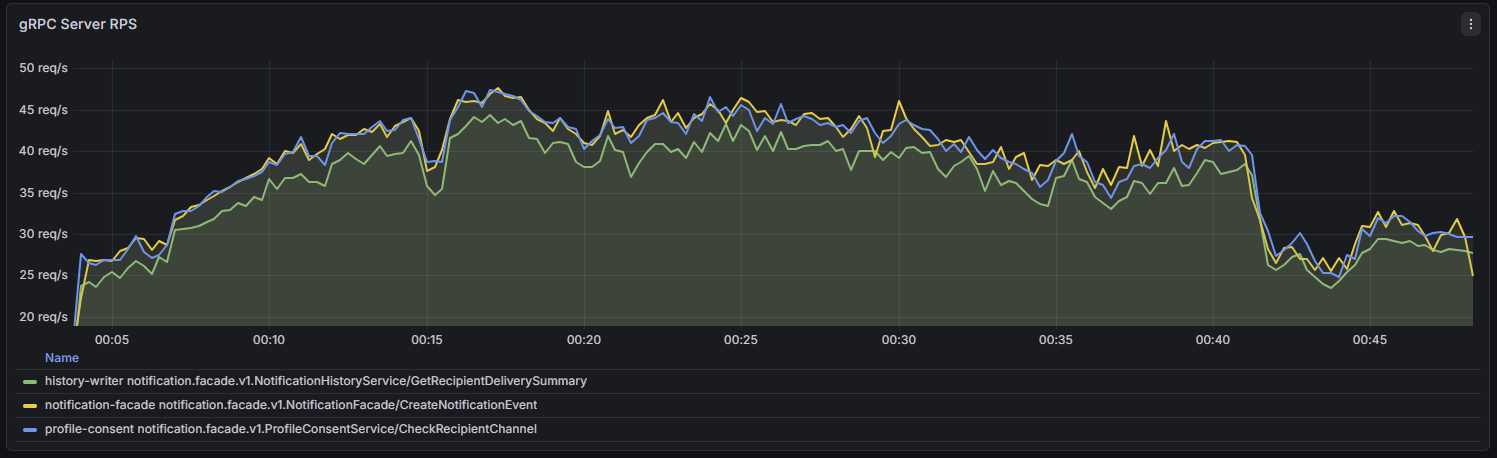
\includegraphics[width=\textwidth]{inc/server_rps.png}
    \caption{Интенсивность серверных gRPC-вызовов в ходе стендового прогона}
    \label{fig:appendix-server-rps}
\end{figure}

\begin{figure}[p]
    \centering
    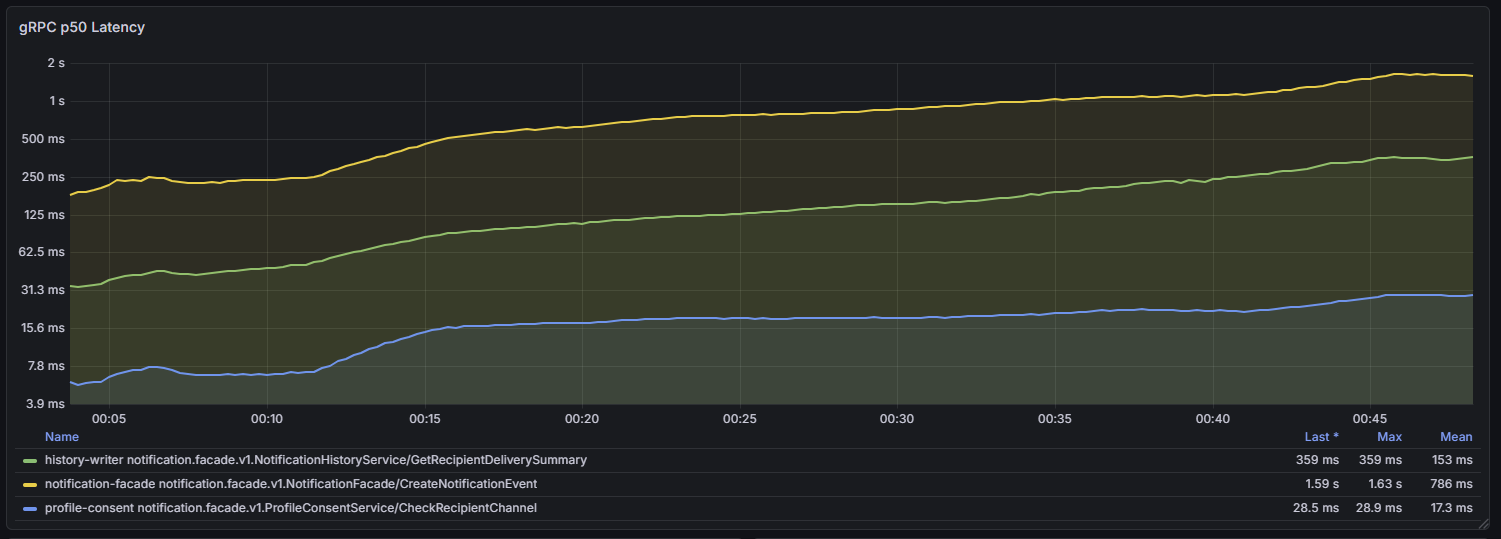
\includegraphics[width=\textwidth]{inc/grpc_p50_lat.png}
    \caption{Медианная задержка ключевых gRPC-вызовов}
    \label{fig:appendix-grpc-p50}
\end{figure}

\begin{figure}[p]
    \centering
    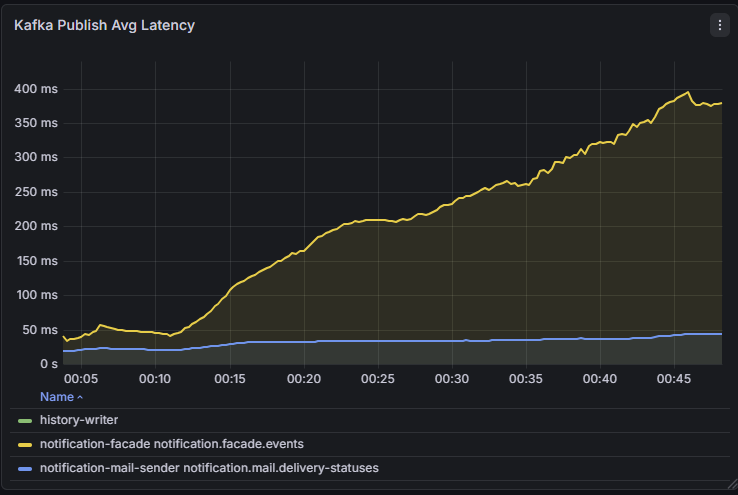
\includegraphics[width=\textwidth]{inc/kafka_avg_latency.png}
    \caption{Средняя задержка публикации сообщений в Kafka}
    \label{fig:appendix-kafka-publish-latency}
\end{figure}

\begin{figure}[p]
    \centering
    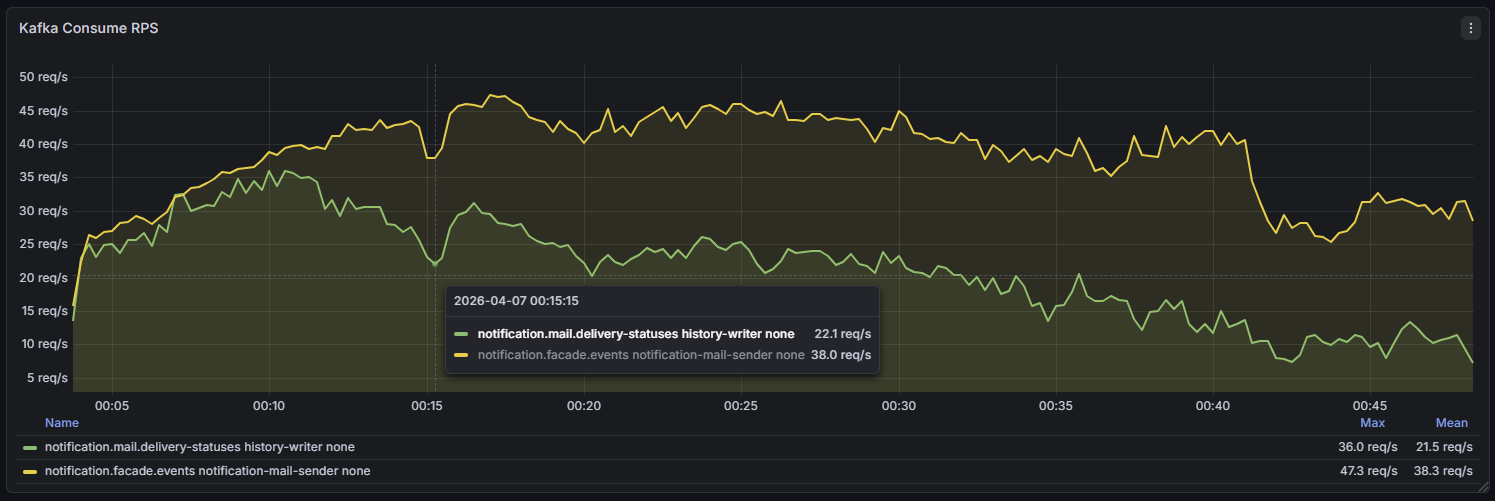
\includegraphics[width=\textwidth]{inc/kafka_consume_rps.png}
    \caption{Интенсивность потребления Kafka-сообщений на основных потребителях}
    \label{fig:appendix-kafka-consume-rps}
\end{figure}

\clearpage

Интерпретация приведённых артефактов выполняется в основной главе о тестировании.
В рамках приложения они сохраняются как подтверждение того, что:
\begin{enumerate}
    \item входные gRPC-вызовы фасада и профильного сервиса наблюдаемы по интенсивности и задержке;
    \item producer-операции Kafka отражаются в метриках времени публикации;
    \item consumer-операции sender-сервисов и history-сервиса наблюдаемы как по RPS, так и по времени обработки;
    \item метрики пригодны для сопоставления стадий одного и того же потока данных.
\end{enumerate}

    \appendixsection{Допущения, ограничения и проверка полноты рукописи}
\label{app:assumptions}

\subsection{Проверка полноты обязательных частей}

Состав подготовленной рукописи проверен по обязательным элементам ВКР. Результат
сведён в таблицу~\ref{tab:appendix-completeness-check}.

\begin{table}[h]
    \centering
    \footnotesize
    \renewcommand{\arraystretch}{1.15}
    \caption{Проверка полноты обязательных частей ВКР}
    \label{tab:appendix-completeness-check}
    \begin{tabular}{|L{0.34\textwidth}|L{0.14\textwidth}|L{0.38\textwidth}|}
        \hline
        \textbf{Обязательная часть} & \textbf{Статус} & \textbf{Комментарий} \\
        \hline
        Титульный лист & Есть & Формируется средствами шаблона diploma. \\
        \hline
        Реферат & Есть & Подготовлен как отдельный файл главы. \\
        \hline
        Содержание & Есть & Формируется автоматически. \\
        \hline
        Введение & Есть & Содержит актуальность, цель, задачи, объект и предмет. \\
        \hline
        Аналитическая глава & Есть & Включает анализ предметной области и обоснование выбора технологий. \\
        \hline
        Постановка задачи и требования & Есть & Включены в аналитическую главу отдельным подразделом. \\
        \hline
        Проектирование архитектуры & Есть & Описаны сервисы, потоки данных, надёжность и безопасность. \\
        \hline
        Моделирование данных & Есть & Описано в главе реализации и приложении. \\
        \hline
        Описание API/контрактов & Есть & Вынесено в главу реализации и приложение с контрактами сервисного взаимодействия. \\
        \hline
        Реализация & Есть & Отражены реальные сервисы и фактический кодовый пайплайн. \\
        \hline
        Тестирование & Есть & Описаны методика, критерии успешности и артефакты наблюдаемости. \\
        \hline
        Экономическая часть / безопасность & Есть & Выполнена качественная оценка и анализ рисков. \\
        \hline
        Заключение & Есть & Сформулированы результаты и направления развития. \\
        \hline
        Список источников & Есть & Оформляется через biblatex. \\
        \hline
        Приложения & Есть & Добавлены приложения по контрактам, Kafka, данным и наблюдаемости. \\
        \hline
        Задание на ВКР & Требует внешнего документа & См. допущение ниже. \\
        \hline
        Календарный план & Требует внешнего документа & См. допущение ниже. \\
        \hline
    \end{tabular}
\end{table}

\subsection{Критические допущения и ограничения}

\assumption{В текущий LaTeX-проект не включены отдельные файлы задания на ВКР и
календарного плана. Согласно используемому шаблону института эти документы
оформляются как внешние материалы и должны быть приложены к итоговому комплекту
работы отдельно.}

\assumption{Текущая кодовая база реализует полноценные sender-сервисы только для
каналов электронной почты и SMS. Канал push присутствует в модели профиля
получателя и может быть развит в дальнейшем, но отдельный push-sender в проекте
на момент подготовки отчёта отсутствует.}

\assumption{В демонстрационном профиле текущей реализации часть gRPC-сервисов и
клиентов работает без обязательной аутентификации, а Kafka и отдельные gRPC-клиенты
используют plaintext-транспорт. Для промышленного внедрения требуется включить
TLS, сервисную аутентификацию и централизованное управление секретами.}

\assumption{Часть адаптеров доставки может работать в тестовом режиме log-only
или через логирующий gateway. Это позволяет верифицировать программный пайплайн,
но не заменяет отдельную промышленную проверку реальных внешних провайдеров.}

\assumption{Экономическая глава выполнена как качественная оценка, поскольку в
составе репозитория отсутствуют утверждённые числовые исходные данные, необходимые
для полного нормативного калькуляционного расчёта.}

\subsection{Проверка целостности текста}

При доработке рукописи были дополнительно проверены следующие аспекты:
\begin{enumerate}
    \item единообразие терминов событие, запуск доставки, канальная доставка;
    \item отсутствие в основном тексте утверждений о несуществующем push-sender;
    \item согласованность описания data flow с фактическими gRPC- и Kafka-контрактами;
    \item наличие источников для обзорных и теоретических положений;
    \item наличие выводов по каждой основной главе.
\end{enumerate}


\end{document}
